%% March 2018
%%%%%%%%%%%%%%%%%%%%%%%%%%%%%%%%%%%%%%%%%%%%%%%%%%%%%%%%%%%%%%%%%%%%%%%%%%%%
% AGUJournalTemplate.tex: this template file is for articles formatted with LaTeX
%
% This file includes commands and instructions
% given in the order necessary to produce a final output that will
% satisfy AGU requirements, including customized APA reference formatting.
%
% You may copy this file and give it your
% article name, and enter your text.
%
%%%%%%%%%%%%%%%%%%%%%%%%%%%%%%%%%%%%%%%%%%%%%%%%%%%%%%%%%%%%%%%%%%%%%%%%%%%%
% PLEASE DO NOT USE YOUR OWN MACROS
% DO NOT USE \newcommand, \renewcommand, or \def, etc.
%
% FOR FIGURES, DO NOT USE \psfrag or \subfigure.
% DO NOT USE \psfrag or \subfigure commands.
%%%%%%%%%%%%%%%%%%%%%%%%%%%%%%%%%%%%%%%%%%%%%%%%%%%%%%%%%%%%%%%%%%%%%%%%%%%%
%
% Step 1: Set the \documentclass
%
% There are two options for article format:
%
% PLEASE USE THE DRAFT OPTION TO SUBMIT YOUR PAPERS.
% The draft option produces double spaced output.
%

%% To submit your paper:
\documentclass[draft,linenumbers]{agujournal2018}
\usepackage{apacite}
\usepackage{gensymb}
\usepackage{url} %this package should fix any errors with URLs in refs.

%%%%%%%
%\usepackage{trackchanges}
% uncomment the line above to use the TrackChanges package to mark revisions if needed.
% The trackchanges package adds five new LaTeX commands:
%
%  \note[editor]{The note}
%  \annote[editor]{Text to annotate}{The note}
%  \add[editor]{Text to add}
%  \remove[editor]{Text to remove}
%  \change[editor]{Text to remove}{Text to add}
%
% complete documentation is here: http://trackchanges.sourceforge.net/
%%%%%%%

\draftfalse

% Now, type in the journal name: \journalname{<Journal Name>}

% ie, \journalname{Journal of Geophysical Research}
%% Choose from this list of Journals:
%
% JGR-Atmospheres
% JGR-Biogeosciences
% JGR-Earth Surface
% JGR-Oceans
% JGR-Planets
% JGR-Solid Earth
% JGR-Space Physics
% Global Biochemical Cycles
% Geophysical Research Letters
% Paleoceanography
% Radio Science
% Reviews of Geophysics
% Tectonics
% Space Weather
% Water Resource Research
% Geochemistry, Geophysics, Geosystems
% Journal of Advances in Modeling Earth Systems (JAMES)
% Earth's Future
% Earth and Space Science
% Geohealth
%

\journalname{JGR-Oceans}


\begin{document}

%  Title
%
% (A title should be specific, informative, and brief. Use
% abbreviations only if they are defined in the abstract. Titles that
% start with general keywords then specific terms are optimized in
% searches)
%
%% ------------------------------------------------------------------------ %%

% Example: \title{This is a test title}

\title{The Seasonal Cycle of Significant Wave Height in the Ocean:  Local vs Remote Forcing}

%% ------------------------------------------------------------------------ %%
%
%  AUTHORS AND AFFILIATIONS
%
%% ------------------------------------------------------------------------ %%

% Authors are individuals who have significantly contributed to the
% research and preparation of the article. Group authors are allowed, if
% each author in the group is separately identified in an appendix.)

% List authors by first name or initial followed by last name and
% separated by commas. Use \affil{} to number affiliations, and
% \thanks{} for author notes.
% Additional author notes should be indicated with \thanks{} (for
% example, for current addresses).

% Example: \authors{A. B. Author\affil{1}\thanks{Current address, Antartica}, B. C. Author\affil{2,3}, and D. E.
% Author\affil{3,4}\thanks{Also funded by Monsanto.}}

\authors{Luke Colosi\affil{1}, Ana B. Villas B\^oas\affil{1}, Sarah T. Gille\affil{1}}


% \affiliation{1}{Scripps Institution of Oceanography, La Jolla, California}
% \affiliation{2}{Second Affiliation}
% \affiliation{3}{Third Affiliation}
% \affiliation{4}{Fourth Affiliation}

\affiliation{1}{Scripps Institution of Oceanography, La Jolla, California}
%(repeat as many times as is necessary)

%% Corresponding Author:
% Corresponding author mailing address and e-mail address:

% (include name and email addresses of the corresponding author.  More
% than one corresponding author is allowed in this LaTeX file and for
% publication; but only one corresponding author is allowed in our
% editorial system.)

% Example: \correspondingauthor{First and Last Name}{email@address.edu}

\correspondingauthor{Sarah T. Gille}{sgille@ucsd.edu}
\correspondingauthor{Ana B. Villas B\^oas}{avillasb@ucsd.edu }

%% Keypoints, final entry on title page.

% Example:
% \begin{keypoints}
% \item	List up to three key points (at least one is required)
% \item	Key Points summarize the main points and conclusions of the article
% \item	Each must be 100 characters or less with no special characters or punctuation
% \end{keypoints}

%  List up to three key points (at least one is required)
%  Key Points summarize the main points and conclusions of the article
%  Each must be 100 characters or less with no special characters or punctuation

\begin{keypoints}
\item Analysis of multi-platform cross calibrated satellite altimetry significant wave height and wind speed using annual and semi-annual seasonal cycle model and regional climatologies in eastern boundary regions of ocean basins where local wind anomalies of similar generation mechanics occur
\item  Deviations in SWH climatologies are have high magnitude in northern hemisphere while low magnitude in the southern hemisphere due to local conditions and characteristics of wave field
\item Probability of swell analysis agrees with hypothesis that the deviation in the SWH climatology in eastern boundary regions of ocean basins occurs due to the local wind anomaly generating locally forced waves during the months of spring and summer in the respective hemispheres 
\end{keypoints}

%% ------------------------------------------------------------------------ %%
%
%  ABSTRACT
%
% A good abstract will begin with a short description of the problem
% being addressed, briefly describe the new data or analyses, then
% briefly states the main conclusion(s) and how they are supported and
% uncertainties.
%% ------------------------------------------------------------------------ %%

%% \begin{abstract} starts the second page

\begin{abstract}

Significant wave height (SWH) provides insight about the interactions between the ocean and the atmosphere. In the Northern and Southern Hemispheres, wave heights have been observed to undergo an annual sinusoidal cycle in response to seasonal changes in storm patterns. In the California coast region, local expansion fan wind events lead to deviations in significant wave height during boreal spring and summer. Other coastal regions where supercritical channel flows occur due to coastal topography and atmospheric forcing include eastern boundary regions of ocean basins (EBR). Here, intra-annual variability of surface gravity waves is analyzed globally in SWH and wind speed data, using over two decades of cross calibrated satellite altimeter SWH measurements produced by the Institut fran\c{c}ais de recherche pour l'exploitation de la mer (Ifremer) and cross calibrated multi-platform wind vector analysis data produced by Remote Sensing Systems. The location at which surface waves are generated is used for validation of mechanisms driving wave characteristics. Phasing of the seasonal cycle reveals that the primary hemisphere dominating the wave field has an abrupt and rough boundary through the equatorial region due in part to topography causing shading of waves. In EBRs the fraction of wave variability attributed to local wind events varies depending on local conditions. Global maps of probability of swell based on wave age confirm that EBRs typically have locally forced waves during the spring and summer months.
% 250 word limit for JGR-Oceans; current length is within this limit.
\end{abstract}


%% ------------------------------------------------------------------------ %%
%
%  TEXT
%
%% ------------------------------------------------------------------------ %%

%%% Suggested section heads:
% \section{Introduction}
%
% The main text should start with an introduction. Except for short
% manuscripts (such as comments and replies), the text should be divided
% into sections, each with its own heading.

% Headings should be sentence fragments and do not begin with a
% lowercase letter or number. Examples of good headings are:

% \section{Materials and Methods}
% Here is text on Materials and Methods.
%
% \subsection{A descriptive heading about methods}
% More about Methods.
%
% \section{Data} (Or section title might be a descriptive heading about data)
%
% \section{Results} (Or section title might be a descriptive heading about the
% results)
%
% \section{Conclusions}


\section{Introduction}

Surface gravity waves are fundamental to our understanding of the interactions between the ocean and atmosphere. Gravity waves are commonly categorized by wave period and generation mechanism \cite{munk1951origin} into a spectrum of ocean waves. In this study, we investigate ordinary gravity waves, which are classified as having wave periods between 1 to 30 seconds and being predominantly generated by wind. This type of surface gravity wave is involved in the exchange of fluid properties including momentum, heat, gasses and energy between the atmosphere and the ocean \cite{cavaleri2012wind}. Over the past half century, satellite remote sensing has revolutionized the way scientists measure and quantify these waves temporally and spatially over the entire global. With the use of satellite altimetry and radiometers or scatterometers, sea surface height and wind speed respectively have been able to be measured on a global scale and over large time periods with spatial resolution on the order of 100km along swath or altimeter footprint on ocean surface. From these satellite observations, the bulk parameter called significant wave height (SWH) may be computed. SWH is defined as the average crest-to-tough height of the 1/3 highest waves within the wave field or as four times the standard deviation of the sea surface elevation \cite{ardhuin2015ocean}. 

Significant wave height (SWH) is an appropriate metric for expressing quantitatively the interaction between the atmosphere and ocean. This interaction in its simplest form consists of near surface wind blowing over an area of ocean for a certain duration leading to a transfer of momentum from the atmosphere into the ocean. This consequently generates ordinary surface gravity waves. Due to the seasonality of storm systems that generate these winds, SWH varies seasonally, with higher values in winter and lower values in summer months. This therefore gives SWH time series sinusoidal variability with a period of approximately 365 days or 12 months which is referred to as the seasonal or annual cycle. This annual cycle accounts for a large percent of variability present in SWH time series for the majority of the ocean as investigated by \citet{echevarria2019seasonal} through principal component analysis of global wind wave hindcast developed by the Centre for Australian Weather and Climate Research (CAWCR). They found that the first two empirical orthogonal functions accounted for $>90\%$ of the variation present in the seasonal climatology time series \cite{echevarria2019seasonal}.  

However, SWH can deviate from a sinusoidal annual cycle for a wide variety of reasons linked to atmospheric forcing on meso and sub-mesoscales. \citet{villas2017characterization} analyzed a distinct deviation occur in the California coast region due to a local wind phenomena call expansion fan winds \cite{winant1988marine}. This deviation is characterized as an increase or simply a bump in SWH due to local wind events generating locally forced waves during the spring and early summer months. The California coast is classified as a eastern boundary current region (EBR) based on the well-known atmospheric conditions and resulting ocean-atmospheric interactions. One example being surface current divergence in the Ekman layer over the continental shelf produce from alongshore prevailing winds cause Ekman suction or upwelling to be set in motion in the interior of the ocean which supplies an abundance of nutrient rich water towards the ocean surface to support a diverse and numerous marine ecosystem \cite{marchesiello2003equilibrium}. These same atmospheric conditions also bring about other physical phenomena. 
%In the Northwest pacific close to the North American coastline, frequently a high pressure system in geostrophic balance with the Coriolis force generates winds circulating anticyconlically southwards down the coastline. Taking a closer view at the california coast...
During boreal spring and summer, the northwest Pacific Ocean frequently has a high pressure system sitting just off the coast of northern California and Oregon. This high pressure system is adjacent to a low pressure thermal low over the western US. From the balance between the pressure gradient force pointing from the high to low pressure systems and the Coriolis force in the atmosphere counteracting this force, an anticyclonic geostrophic atmospheric flow is generated which drives southward winds along the coast of California. Due to the coast mountain range in the northern and central parts of California and an inversion layer capping the marine layer, a boundary interface just below the height of the coastal mountain range, a supercritical wind channel forms. This wind channel polarizes the wind direction parallel to the coast. In addition, wind speed increases as the wind passes along the coast through capes which are swooping bays found along the coast of California. This amplification of wind speed and polarized direction generates wind speeds greater than expected in the geostrophic wind field predictions. These strong wind blowing down the California coast influences the wave field significantly. During the spring months, an increase in SWH is observed in climatological time series analysis and has been directly linked to the local expansion fan wind event which produced these locally forced waves. Locally generated waves can be characterized in the SWH seasonal cycle as having short period or high frequency when compared to remotely forced waves. This results in choppy surface ocean conditions near the coast. 

%As the predominant northerly (blows from north to south) winds off the California coast in the spring and summer time travels south (due to a high pressure system off the pacific northwest and a thermal low (low pressure system) in the west US region) , the coastal topography and a low-level inversion capping the marine layer create a boundary interface below the height of the coastal mountain range causes an amplification in wind speed (greater than geostrophic wind field predictions) and wind direction to be parallel to the coastline in what is know as a supercritical channel flow in the atmosphere. 

This same supercritical channel flow has been hypothesized by  \citet{winant1988marine} to be present in other EBRs in ocean basins that have coastal topography and atmospheric conditions similar to California. These regions include the west coast of Australia, the coast of Nigeria in southern Africa, the coast of Chile, the southern Caribbean sea and the northwest coast of Africa near Morocco, and in the Arabian sea near the tip of Somalia. 

By analyzing intra-annual variability of SWH for surface gravity waves and wind speed (WSP) on a global scale from 1993 to 2015 using active satellite remote sensing, we investigate EBRs to determine if the same seasonal cycle deviation as in the California Coastal region is present and if a corresponding maximum in wind speed seasonal cycle is correlated to the SWH deviation. In addition, the structural distribution of the characteristic of the seasonal and semi-seasonal cycle on a global scale is explored in order to give insight into the general forcing mechanisms and characteristics of the wave field influencing these deviations in SWH\@. In order to justify that SWH during the spring months in these EBRs are locally forced, wave age can be used for separating growing seas from fully developed seas for a collocated observed wind speed and SWH measurement.

This paper is organized as follows.  Section 2 explains the data sets used to conduct the time series analysis of global SWH data and the limitations of our analysis.  Section 3 explores the general characteristic of the annual and semi-annual SWH models for the entire time series globally as well as regional climatologies in order to demonstrate the correlation between the deviations in the seasonal cycle and the maximum in the wind speed seasonal cycle.  Section 4 uses wave age in order to illustrate that SWH measurements during the spring months within EBRs are observing locally forced wave rather than remotely forced wave justifying the claim that local wind events are causing the deviation in the seasonal cycle.  Section 5 summarizes conclusions.

\section{Methods}

\subsection{Remotely sensed Data}

This study makes use of separate multi-satellite remote sensing products for waves and wind.   

Wave data used in this study are drawn from two decades of cross-calibrated satellite altimeter significant wave height measurements produced by the Institut fran\c{c}ais de recherche pour l'exploitation de la mer (Ifremer).  Ifremer's along track cross calibrated SWH altimeter data was collected from multiple near pole non-sun synchronous satellites over the time period of 1 January 1993 to 31 December 2015. The along track data were binned onto a 1$^{\circ}$ by 1$^{\circ}$ spatial grid with 1-day temporal resolution. Satellites contributing to the analysis include ERS-1\&2, TOPEX-Poseidon, GEOSAT Follow-ON (GFO), Jason-1, Jason-2, ENVISAT, Cryosat and SARAL AltiKa \cite{Queffeulou2017Global}. To enhance the quality of SWH observations, data screening based on multiple flags and uncertainty of measurements to determine the reliability and viability of each data point was performed. Ifremer SWH data are corrected to agree with in situ buoy observations.

Wind data for this study are from the cross calibrated multi-platform version 2 wind vector analysis data (CCMP2) produced by Remote Sensing Systems. CCMP2's data product is released on a 0.25$^{\circ}$ by 0.25$^{\circ}$ spatial grid with 6 hourly temporal resolution. For this analysis, we averaged CCMP2 winds to a 1$^{\circ}$ by 1$^{\circ}$ spatial resolution and 1 day temporal resolution in order to match the Ifremer data set. The CCMP2 product incorporates measurements from active scatterometers, passive radiometers, in situ buoys, and modelled wind velocity data \cite{Atlas2011Remote}. CCMP reports wind in zonal and meridional components \cite{Atlas2011Remote}, which are used to compute WSP. 

For the climatological analysis, monthly data products of SWH and WSP were then obtained by averaging over each month throughout the time period. Ifremer's along track daily data set can be found on the servers ftp://ftp.ifremer.fr/ifremer/cersat/products/swath/altimeters/waves where this Ifremer data is public available. In addition, the CCMP2 6 hourly wind vector data set can be found on ftp://ftp.remss.com/ccmp/v02.0 which remote sensing systems maybe accessed at  www.remss.com. 

The Ifremer SWH product is not co-located temporally with the CCMP2 wind product; typical  time differences are on the order of 6 hours. For point-to-point analysis, this would present a major obstacle due to the fact that the sea state including wave height or SWH and atmospheric conditions including WSP are highly variable on time scales of minutes to hours, meaning that SWH and WSP can change significantly within a 6 hour period. Therefore, the WSP measurement at a given location could have no correlation at all to a SWH measurement taken 6 hours later at the same location. The analysis done in this study focuses on monthly averaged SWH and WSP.

%Is it okay that I am leave the discussion about WW3 CFSR data until the discussion section? Or should I bring it up in this section?

\subsection{Annual and Semi-Annual Model and Regional Climatology Analysis}

In order to analyze the seasonal cycle of SWH and WSP, at each grid point, we least-squares fitted SWH and WSP with annual and semi-annual sinusoidal cycles: 
 \begin{equation}
     \mbox{\rm model} = x_1 + x_2\times\sin\left(\frac{2{\pi}t}{T}\right) +  x_3\times\cos\left(\frac{2{\pi}t}{T}\right) + x_4\times\sin\left(\frac{4{\pi}t}{T}\right) + x_5\times\cos\left(\frac{4{\pi}t}{T}\right).
 \end{equation}
Here, T is the duration of the annual cycle (12 months), t is time, and $x_n$ are coefficients for the SWH or WSP model. A linear trend within the SWH and wind speed time series was not accounted for within our analysis nor was any detrending performed on the data assuming that linear trend within the data set were negligible or unreal artifact of the cross calibrated multi-platform data sets.

The characteristics used to evaluate and compare the seasonal cycles spatially were the amplitude and phase constant. In order to evaluate the goodness of fit of the model, the root mean square of the residual and coefficient of determination was used. The residual is defined as the difference between the seasonal cycle model and the observed data. This method is a rudimentary method of quantifying how well the seasonal cycle model fit the observed data and is biased to have high residue in regions with high temporal variability.
\begin{equation}
    \mbox{\rm residual} = \mbox{\rm model} - \mbox{\rm data} 
\end{equation}
\begin{equation}
    \mbox{\rm Root Mean Square Error} = \sqrt{\langle \mbox{\rm residual}^2\rangle} 
\end{equation}
The coefficient of determination is the percent of variation of the data explained by the model and is calculated by taking the ratio of the summed squared error between each data point and the corresponding modelled data divided by the difference between the data point and the mean value of the data.
\begin{equation}
 r^{2} = 1 - \frac{\rm SS_{res}}{\rm SS_{total}} = 1- \frac{\sum (y_i - f_i)}{\sum (y_i - \overline{y})}
 \end{equation}
Here $f$ is equivalent to the least square fit model. The coefficient of determination provides a more robust quantification of the goodness of fit of the model. For the amplitude and the phase constant of the annual and semi-annual cycle, these characteristics were determined by the following equations
 \begin{eqnarray}
     annual\;amplitude & = & \sqrt{x_2^{2} + x_3^{2}}\\
    semi-annual\;amplitude & = & \sqrt{x_4^{2} + x_5^{2}}\\
     annual\;phase & = & \arctan{\left(\frac{x_3}{x_2}\right)} \\
    semi-annual\;phase & = & \arctan{\left(\frac{x_5}{x_4}\right)}\\
 \end{eqnarray}
For the climatological analysis within EBRs, all grid points within 4$^{\circ}$ by 4$^{\circ}$ square regions were spatially and monthly averaged in order to obtain SWH and WSP climatologies for the region to compare the SWH deviation with the maximum of the WSP. The 4$^{\circ}$ by 4$^{\circ}$ regions were picked by looking at seasonally averaged WSP maps within EBRs for regions that had anomalously high WSP and small spatial WSP gradients as seen in Fig~\ref{reg_clima_nh}. Small spatial gradients and a decently sized regions to spatially average data were favorable for obtaining smooth climatologies. Through the combination of these characteristics, many inferences about the underlying dynamics influencing the climatology of specific regions were able to be made. 

Seasonal progression maps of the first two statistical moments for Ifremer SWH and CCMP2 WSP data are computed in order to gain insight into the seasonal evolution and variability of the data.

\subsection{Limitations of Data}

The data used in this study have limitations associated with retrieval methods and with multi-satellite intercalibration in order to obtain a continuous or ``gap free" temporal or spatial data set for SWH and WSP. 

In order to obtain accurate satellite altimetry data, corrections must be made for the sea surface elevation measurement which include instrument, atmospheric refraction, and sea-state bias corrections as well as external geophysical adjustments \cite{fu2000satellite}. All these sources of error introduce a certain degree of uncertainty and unreliability with a satellite's measurements.  
%can be introduced from two main sources: the above ground attenuation of the radar signal from environmental factors and sea state effects. 
In brief, the environmental factors attributed to introducing systematic and random error into the data set includes atmospheric attenuation and refraction from clouds and rain. On-board satellite error include flight trajectory and location precision of satellite during orbit, drift error of sensors and footprint size, and location where measurements are being taken. For all satellite mission, each satellite is on a non-sun synchronous near pole orbit in order for the satellites to collect data a each grid point throughout the year at different times during the day. This allows the satellite measurements record to be less likely to bias certain sea surface topography structures which tend to occur during a specific time throughout the day. The total sea state bias includes the electromagnetic (EM) and skewness biases. These two errors weaken the reliability of the altimetry measurements of satellites in regions with high wave height or high frequency waves. EM and skewness biases arise from systemic error present in the altimeter's ability to accurately sense the mean sea level within the sea surface height distribution of the satellite's footprint. This is due to the distribution of backscatterers of the incident radiation on the ocean surface. The power of backscattering off a wave facet is proportional to the local radius of curvature \cite{fu2000satellite}. Due to the non-Gaussian distribution of sea surface height, wave troughs have larger radius of curvatures and therefore, high backscatter than wave crests. This biases the sea level (or the mean or media scattering surface) towards the wave troughs \cite{fu2000satellite}. This leads to an underestimation of the sea surface elevation and therefore an underestimation of SWH within wind-sea regions. Wind-sea regions tend to have high wave steepness and small-scale roughness near the wave crests which amplifies the sea state biases introduced to the sea surface height measurement. Corrections of sea state bias for SWH have be applied to the satellite altimetry data, however, the error varying in magnitude based geographically are still present in sea surface height measurements.

In addition, satellite altimetry data in near coastal region on the scales of 100km should be neglected from the analysis due to the spatial extent of the swath of the satellite. The footprint of satellite is on the order of 100km which means that until the foot is covering only the ocean surface, the data can be contaminated by the land. Fortunately, the local wind anomalies persist for several hundreds of kilometer off shore allowing reliable SWH and WSP data satellite data to be recorded. 

%Advances have been made to understand and account for this bias, however there is still a high level of uncertainty of the sea surface elevation. This leads to a higher uncertainty and possibly an underestimation of SWH within wind-sea regions.

This study takes advantage of the global moderate to high spatial and temporal resolution measurements of significant wave height measurements from Ifremer's cross-calibrated multi-satellite mission product to look at the intra-annual variability of the SWH seasonal cycle over a 20 year time period; however, with caution due to the known limitations of the data set coming from the stated environmental and instrumental biases present especially in wind-sea regions.

In addition, this study only focuses on time series analysis of averaged parameters, including SWH, peak frequency (or period) and mean wave direction.   At any given point on earth, these describe only the dominant wave height, frequency, period, and direction of waves within the wave spectrum that is associated with the highest spectral energy or elevation variance \cite{ardhuin2015ocean}. Therefore, weaker but still prevalent signals from swell and wind-sea waves are suppressed in the result as a result of this analysis. \citet{echevarria2019seasonal} highlight this shortcoming of bulk parameters in wave climatology analysis and present a climatological analysis of multimodal directional wave spectrum via principal component analysis of the spectral data from Wave Watch 3 ECMWF reanalysis data. \citet{semedo2011global} also used as well Wave Watch 3 ECMWF reanalysis data in order to analyze the global wave climate . Bulk parameters are used in this analysis with the understanding of its limited ability to full describe all modes present in the wave spectrum. However, this study's results only reflect the analysis of dominant highest spectral energy signal present.

\section{Results}

\subsection{Global Characteristics of Annual and Semi-annual Model and Implications to EBRs}

By considering the time period from January 1st, 1993 to December 31st, 2015, a five parameter model was fitted to each 1$^{\circ}$ by 1$^{\circ}$ degree grid box for monthly averaged daily Ifremer SWH and 6 hourly CCMP2 WSP data sets. From each model, the residual, amplitude, phase, coefficient of determination were computed. The five parameter model accounted for a mean offset, annual cycle and semi-annual cycle of SWH. Therefore, the amplitude and phase for the annual and semi-annual cycles were computed. Figure~\ref{Ifremer_ccmp2_lsf_chars} compares the Ifremer SWH annual and semi-annual cycle amplitude and phase with CCMP2 WSP results.

\begin{figure}[tbh]
\centering
\includegraphics[width=1.0\textwidth]{figs/lsf_characteristics/ccmp2_ifremer_lsf_characteristics_5_par_fit_cbc.png}
\caption{Amplitude of annual cycle for (A) Ifremer SWH and (B) CCMP2; amplitude of semi-annual cycle for (C) Ifremer SWH and (D) CCMP2 WSP; phase of annual cycle for (E) Ifremer SWH and (F) CCMP2 WSP; phase of semi-annual cycle for (G) Ifremer SWH and (H) CCMP2 WSP.  See text for details of computation.}
\label{Ifremer_ccmp2_lsf_chars}
\end{figure}

The annual seasonal cycle phase maps for SWH (Fig.~\ref{Ifremer_ccmp_lsf_chars}E) shows that the phase of the seasonal cycle in the Northern Hemisphere is approximately 6 months out of phase with the Southern Hemisphere, with the timing of maximum waves well aligned with the timing of maximum WSP (Fig.~\ref{Ifremer_ccmp_lsf_chars}F)  This 6-month phase shift illustrates the storm systems' annual frequency and intensity cycles in the mid to high latitudes of the Northern and Southern Hemispheres. This means storms with high wind speeds that blow over larger fetches of ocean form more frequently during winter months and more seldomly with lower wind speeds during summer months. The complementary situation for the southern hemisphere follows the same argument above. This means that the structure of the seasonal cycle in the southern hemisphere is also set by storm patterns and local wind event occurrences. 

%These shifts in phase are illustrated in Figure~\ref{NSH_time_series_comp} by considering the spatially averaged 2 year time series of the northern and southern hemisphere and observing at what times in the year the maximum and minimums in the swh seasonal cycle occur. 

%\begin{figure}[htb]
%\centering
%\includegraphics[width=0.25\textwidth]{figs/supplemental_figs%/SC_NSH_overlap.png}
%\caption{Spatially averaged SWH daily resolution time series for the Northern and Southern hemispheres from January 1st, 2014 to Decemeber 31t, 2015. Hemispheres are designated chosen as being greater than or equal to 10$^{\circ}$N and greater than or equal to 10$^{\circ}$S respectively.}.
%\label{NSH_time_series_comp}
%\end{figure}

%\begin{wrapfigure}{L}{0.2\textwidth}
%\vspace{−12pt}
%\includegraphics[width=0.2\textwidth]{figs/supplemental_figs/SC_NSH_overlap.png}
%\vspace{−20pt}
%\caption{Spatially averaged SWH daily resolution time series for the Northern and Southern hemispheres from January 1st, 2014 to December 31t, 2015. Hemispheres are designated chosen as being greater than or equal to 10$^{\circ}$N and greater than or equal to 10$^{\circ}$S respectively.}
%\end{wrapfigure}

Other features in the SWH annual cycle phase map include higher spatial variability in the Southern Hemisphere than in the Northern Hemisphere, possibly due to the consistently high variance in the mid to high latitudes of the Southern Hemisphere (Fig~\ref{Ifremer_swh_seasonal_var}). In the equatorial region, the dominant phase changes roughly along a line where the amplitude of the seasonal cycle tends towards zero (Fig~\ref{Ifremer_ccmp2_lsf_chars}A). This boundary designates the transition from the seasonal cycle being primarily set by storm system originating in the Northern hemisphere to being primarily set by storm systems originating in the southern hemisphere. This smooth transition is expected in the region where the amplitude tends towards zero. This phase boundary in the Pacific and Atlantic is also known as a swell front \cite{young1999seasonal}  and is the boundary between domains of dominance of swell from each hemisphere and discussed in Semedo et al. 2011 and chen et al. 2013. However, waves propagating from the Northern and Southern Hemispheres coexist superimposed on the wave field at and beyond the swell front. This means that the waves will continue propagating in their respective directions into the opposite hemisphere \cite{echevarria2019seasonal}.

In the tropical Pacific, several abrupt shifts in phase exist between 10$^{\circ}$ and 20$^{\circ}$ south at approximately 180$^{\circ}$E and 145$^{\circ}$W (Figure~\ref{phase_amp_topo_comp}). One explanation for these abrupt phase shifts is island shadowing. Waves from the Southern Ocean propagating northward encounter the topography of Polynesian islands and break and dissipate on the shores facing the direction of the oncoming waves. The opposite side of the island does not encounter any of these remotely or locally forced waves. Therefore, the southern facing sides of these islands are in phase with the Southern Hemisphere seasonal cycle while the northern facing sides of the islands are in phase with the northern hemisphere because they are only exposed to southward traveling waves originating in the Northern Hemisphere. Some waves are able to squeeze between these islands as well. Waves from the Southern Ocean that are able to propagate through the Polynesian islands continue into the northern Pacific. Evidence for this northward propagation can be seen in the slow decrease and a slightly higher phase constant value between the two indentations present on the phase boundary.

%In Figure~\ref{phase_topo_comp}, islands lie around these indentations and there are clear examples of island shadowing occurring at below the indentations at 180$^{\circ}$ east and 145$^{\circ}$ west. These two larger island clusters north facing shores have very little or no exposure at all to waves propagating from southern ocean storms. This cause a small region on the north facing shore to be in phase with the northern hemisphere seasonal cycle such that the region primarily exposed to northern hemisphere remotely forced waves.  

\begin{figure}[htb]
\centering
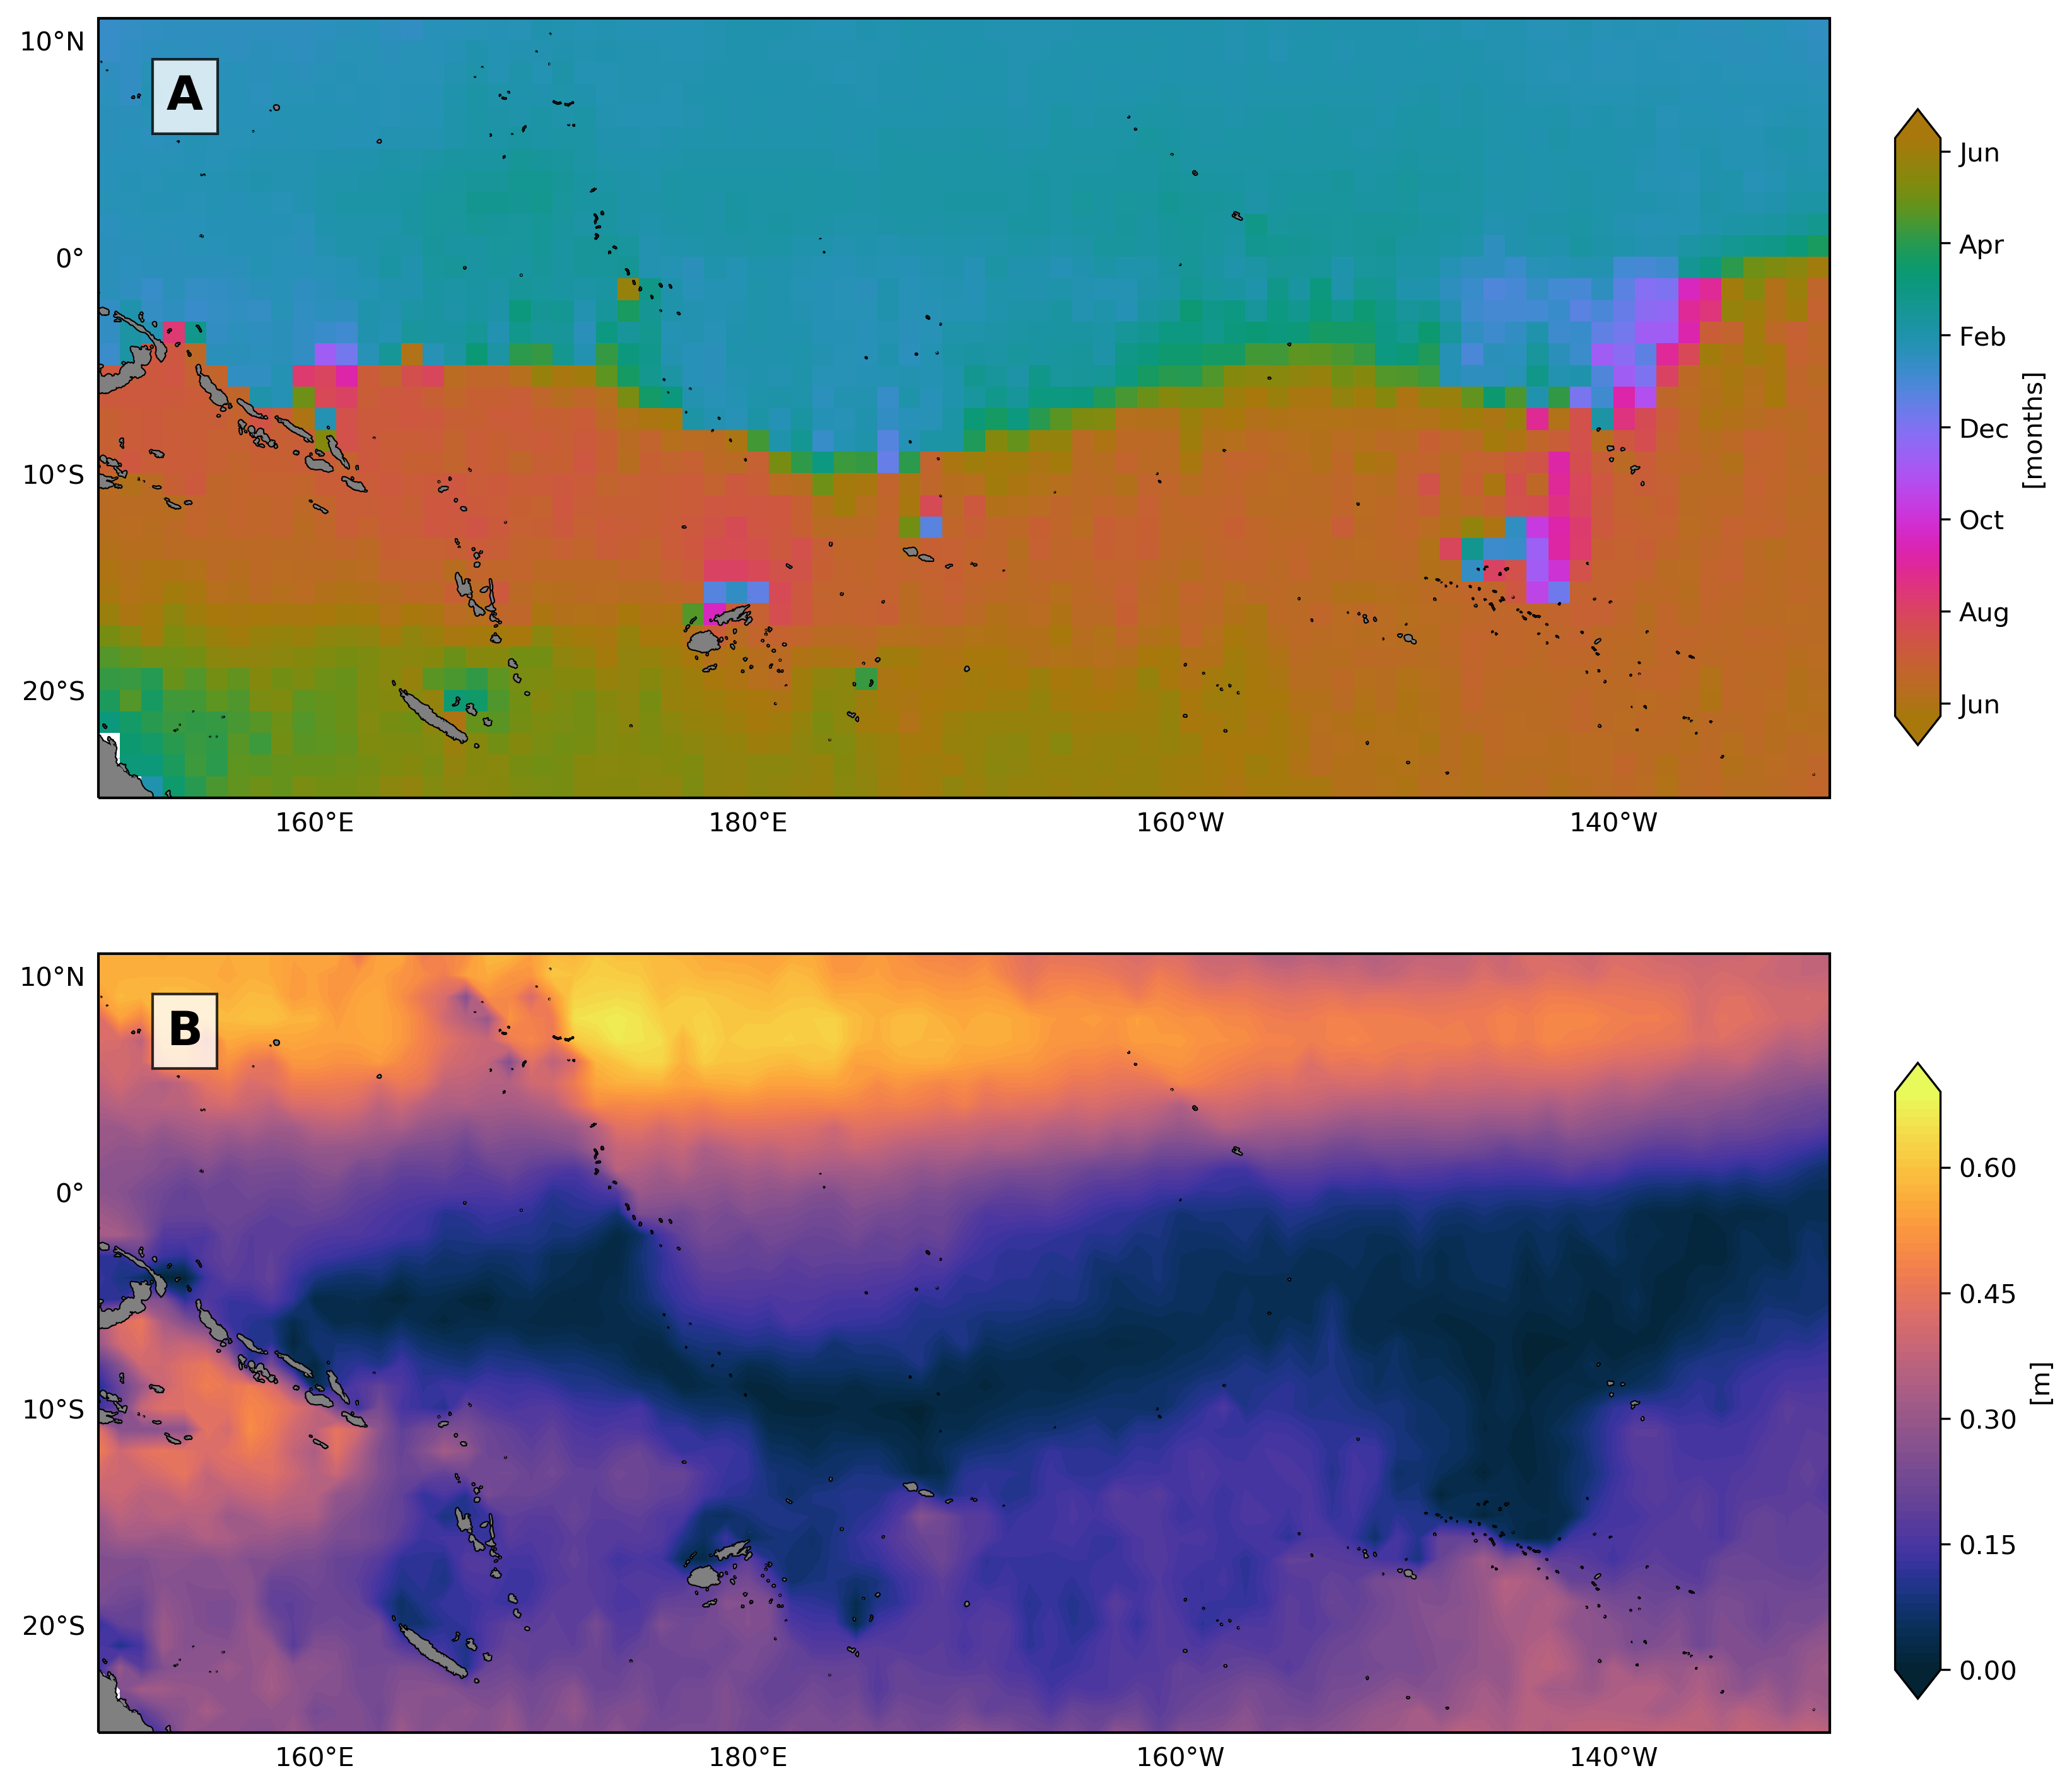
\includegraphics[width=1.0\textwidth]{figs/lsf_characteristics/Phase_amp_topography_overlap.png}
\caption{(A) Ifremer SWH Annual cycle phase map in Polynesian island region illustrating island shadowing, (B) Ifremer SWH annual cycle amplitude map in Polynesian island region }
\label{phase_amp_topo_comp}
\end{figure}

The phase transition from the Northern Hemisphere dominated domain to the Southern Hemisphere dominated domain occurs slightly south of the equator between 5$^{\circ}$ and 10$^{\circ}$S in the west, and it slowly shifts equatorward to the east. Explanations for the geographic location of the boundary are linked to where the amplitude of the seasonal cycle tends to zero. Other explanations include the following. Waves would encounter westward flowing south equatorial current (SEC), south equatorial countercurrent (SECC), the westward north equatorial current (NEC), or the north equatorial countercurrent (NECC). The SEC and SECC are located on average closest to the phase boundary, and they are known to be present between 5$^{\circ}$ and 10 $^{\circ}$S \cite{talley2011descriptive}. The wave-current interactions between waves propagating into this region from the Northern and Southern Hemisphere have no effects of wave propagation when the velocities of the two are orthogonal. In addition, the wave-current interaction is on small scales and would be undetectable in satellite altimeter SWH data when the footprint of the satellite covers several kilometers of sea surface. In addition, the phase boundary of the annual cycle does not line up with the intertropical convergence zone (ITCZ) characterized as a low pressure system with heavy precipitation and deep convection that causes very calm sea surface conditions. These calm sea surface conditions could be thought of as being associated with the low amplitude seasonal cycle region. However, low amplitude does not imply low SWH values because there is a mean value that offsets the SWH seasonal oscillations from zero. By looking at the SWH seasonal mean Fig~\ref{Ifremer_swh_seasonal_mean}, the mean is relatively low, but not the minimum value of the equatorial region. In addition, the intertropical  convergence zone annual migrates between 9$^{\circ}$N in boreal summer and 2$^{\circ}$N in boreal winter in the central Pacific following the warmer hemisphere. This is significantly far from the phase boundary. Wave to wave interactions and non-conservative forcing could possible play a significant role here; however, the angle between the wave group velocity determines significantly how energy and momentum will be distributed throughout the system. By looking at fig~\ref{phase_amp_topo_comp}, we see that islands within this region play a significant role in setting the shape of the minimum annual cycle amplitude region for SWH. Islands outline the near zero contour for amplitude and therefore significantly affect how waves propagate into this region and how those waves will interact with each other. 

Other interesting structures exist in near coastal regions and in the Atlantic. In the Atlantic, there is also a smooth phase boundary transition with one abrupt phase shift close to the western side of the Atlantic. On the western side, the phase boundary is almost vertical following a line of constant latitude. This dynamic boundary also occurs in the zero amplitude SWH seasonal cycle region and is slightly below the equator. In addition, just off the coast of Mexico, there is an out of phase region that is close to the near zero amplitude region. These other structures will be left for further research.

\begin{figure}[tbh]
\centering
  \begin{minipage}{.5\textwidth}
    \centering
    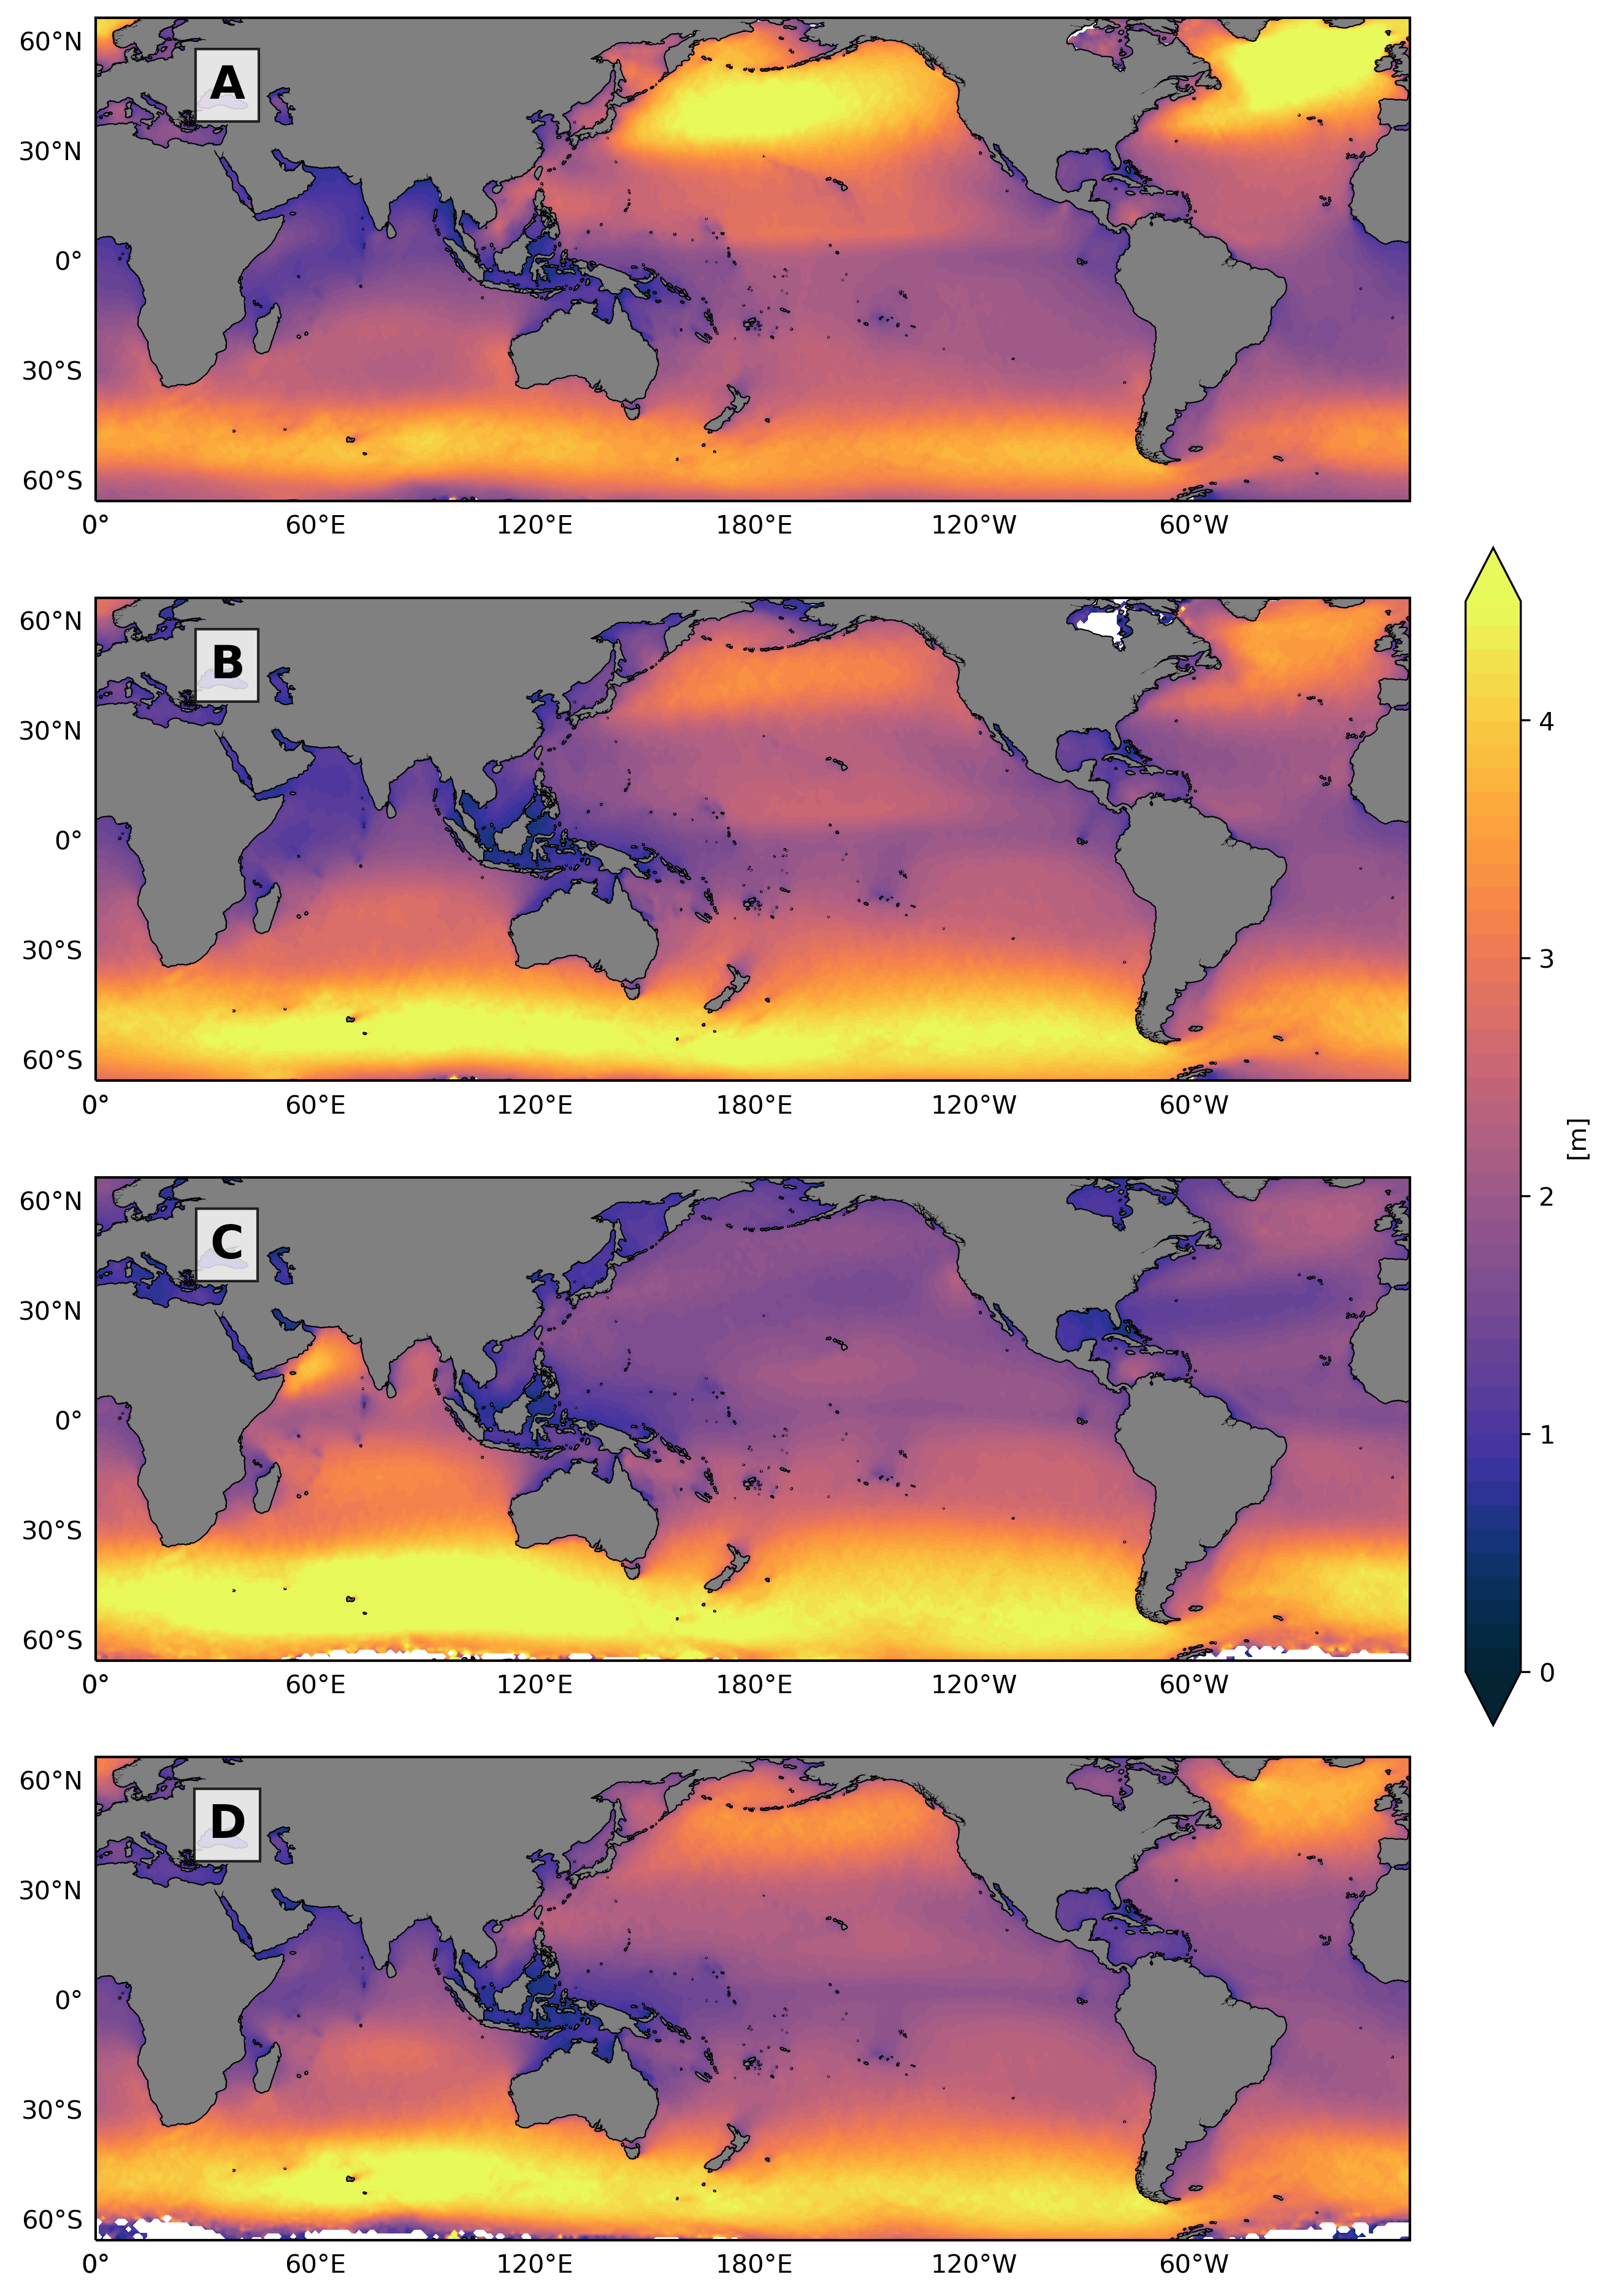
\includegraphics[width=0.5\textwidth]{figs/statistical_moments/Ifremer_p1_seasonal_mean.png}
    \caption{Ifremer SWH Seasonal Mean}
    \label{Ifremer_swh_seasonal_mean}
  \end{minipage}%
  \begin{minipage}{.5\textwidth}
    \centering
    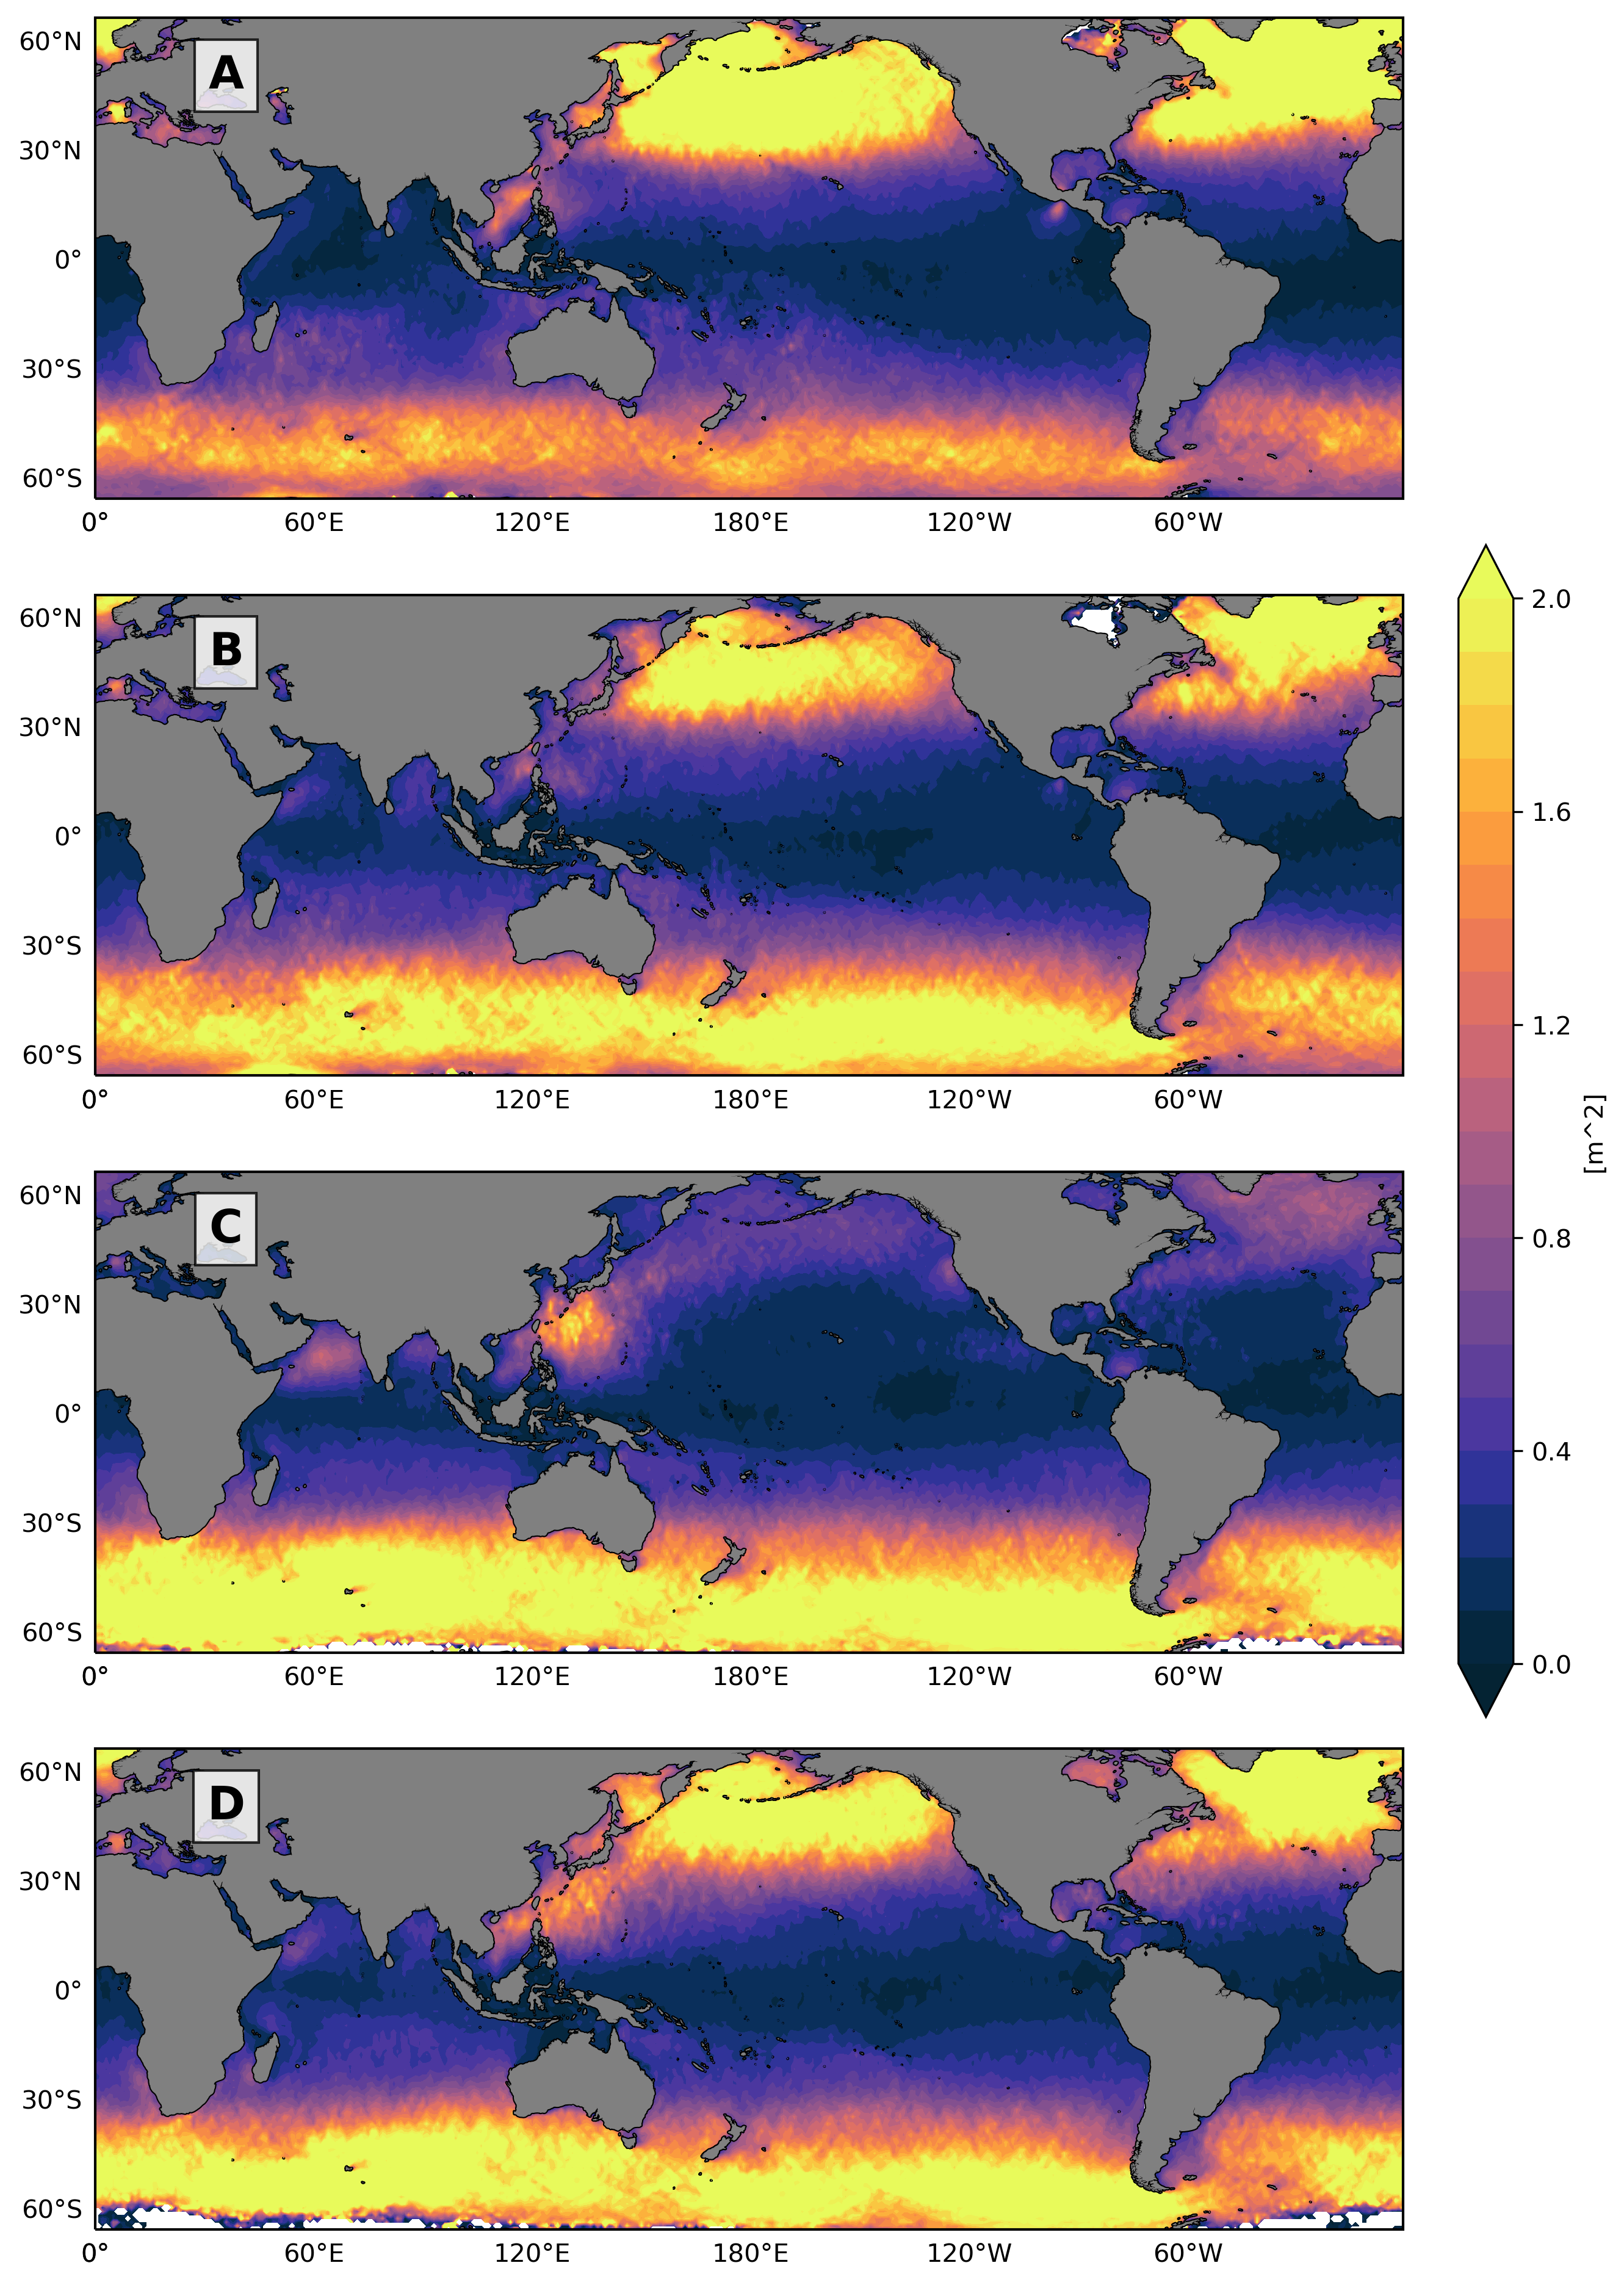
\includegraphics[width=0.5\textwidth]{figs/statistical_moments/Ifremer_p1_seasonal_var.png}
    \caption{Ifremer SWH Seasonal Variance}
    \label{Ifremer_swh_seasonal_var}
\end{minipage}
%\caption{Ifremer SWH First and Second Statistical Moments seasonal progression with A) December through February, B) March through May, C) June %through August, and D) September through November}
\label{Ifremer_swh_seasonal_pro}
\end{figure}

\begin{figure}[tbh]
  \begin{minipage}{.5\textwidth}
    \centering
    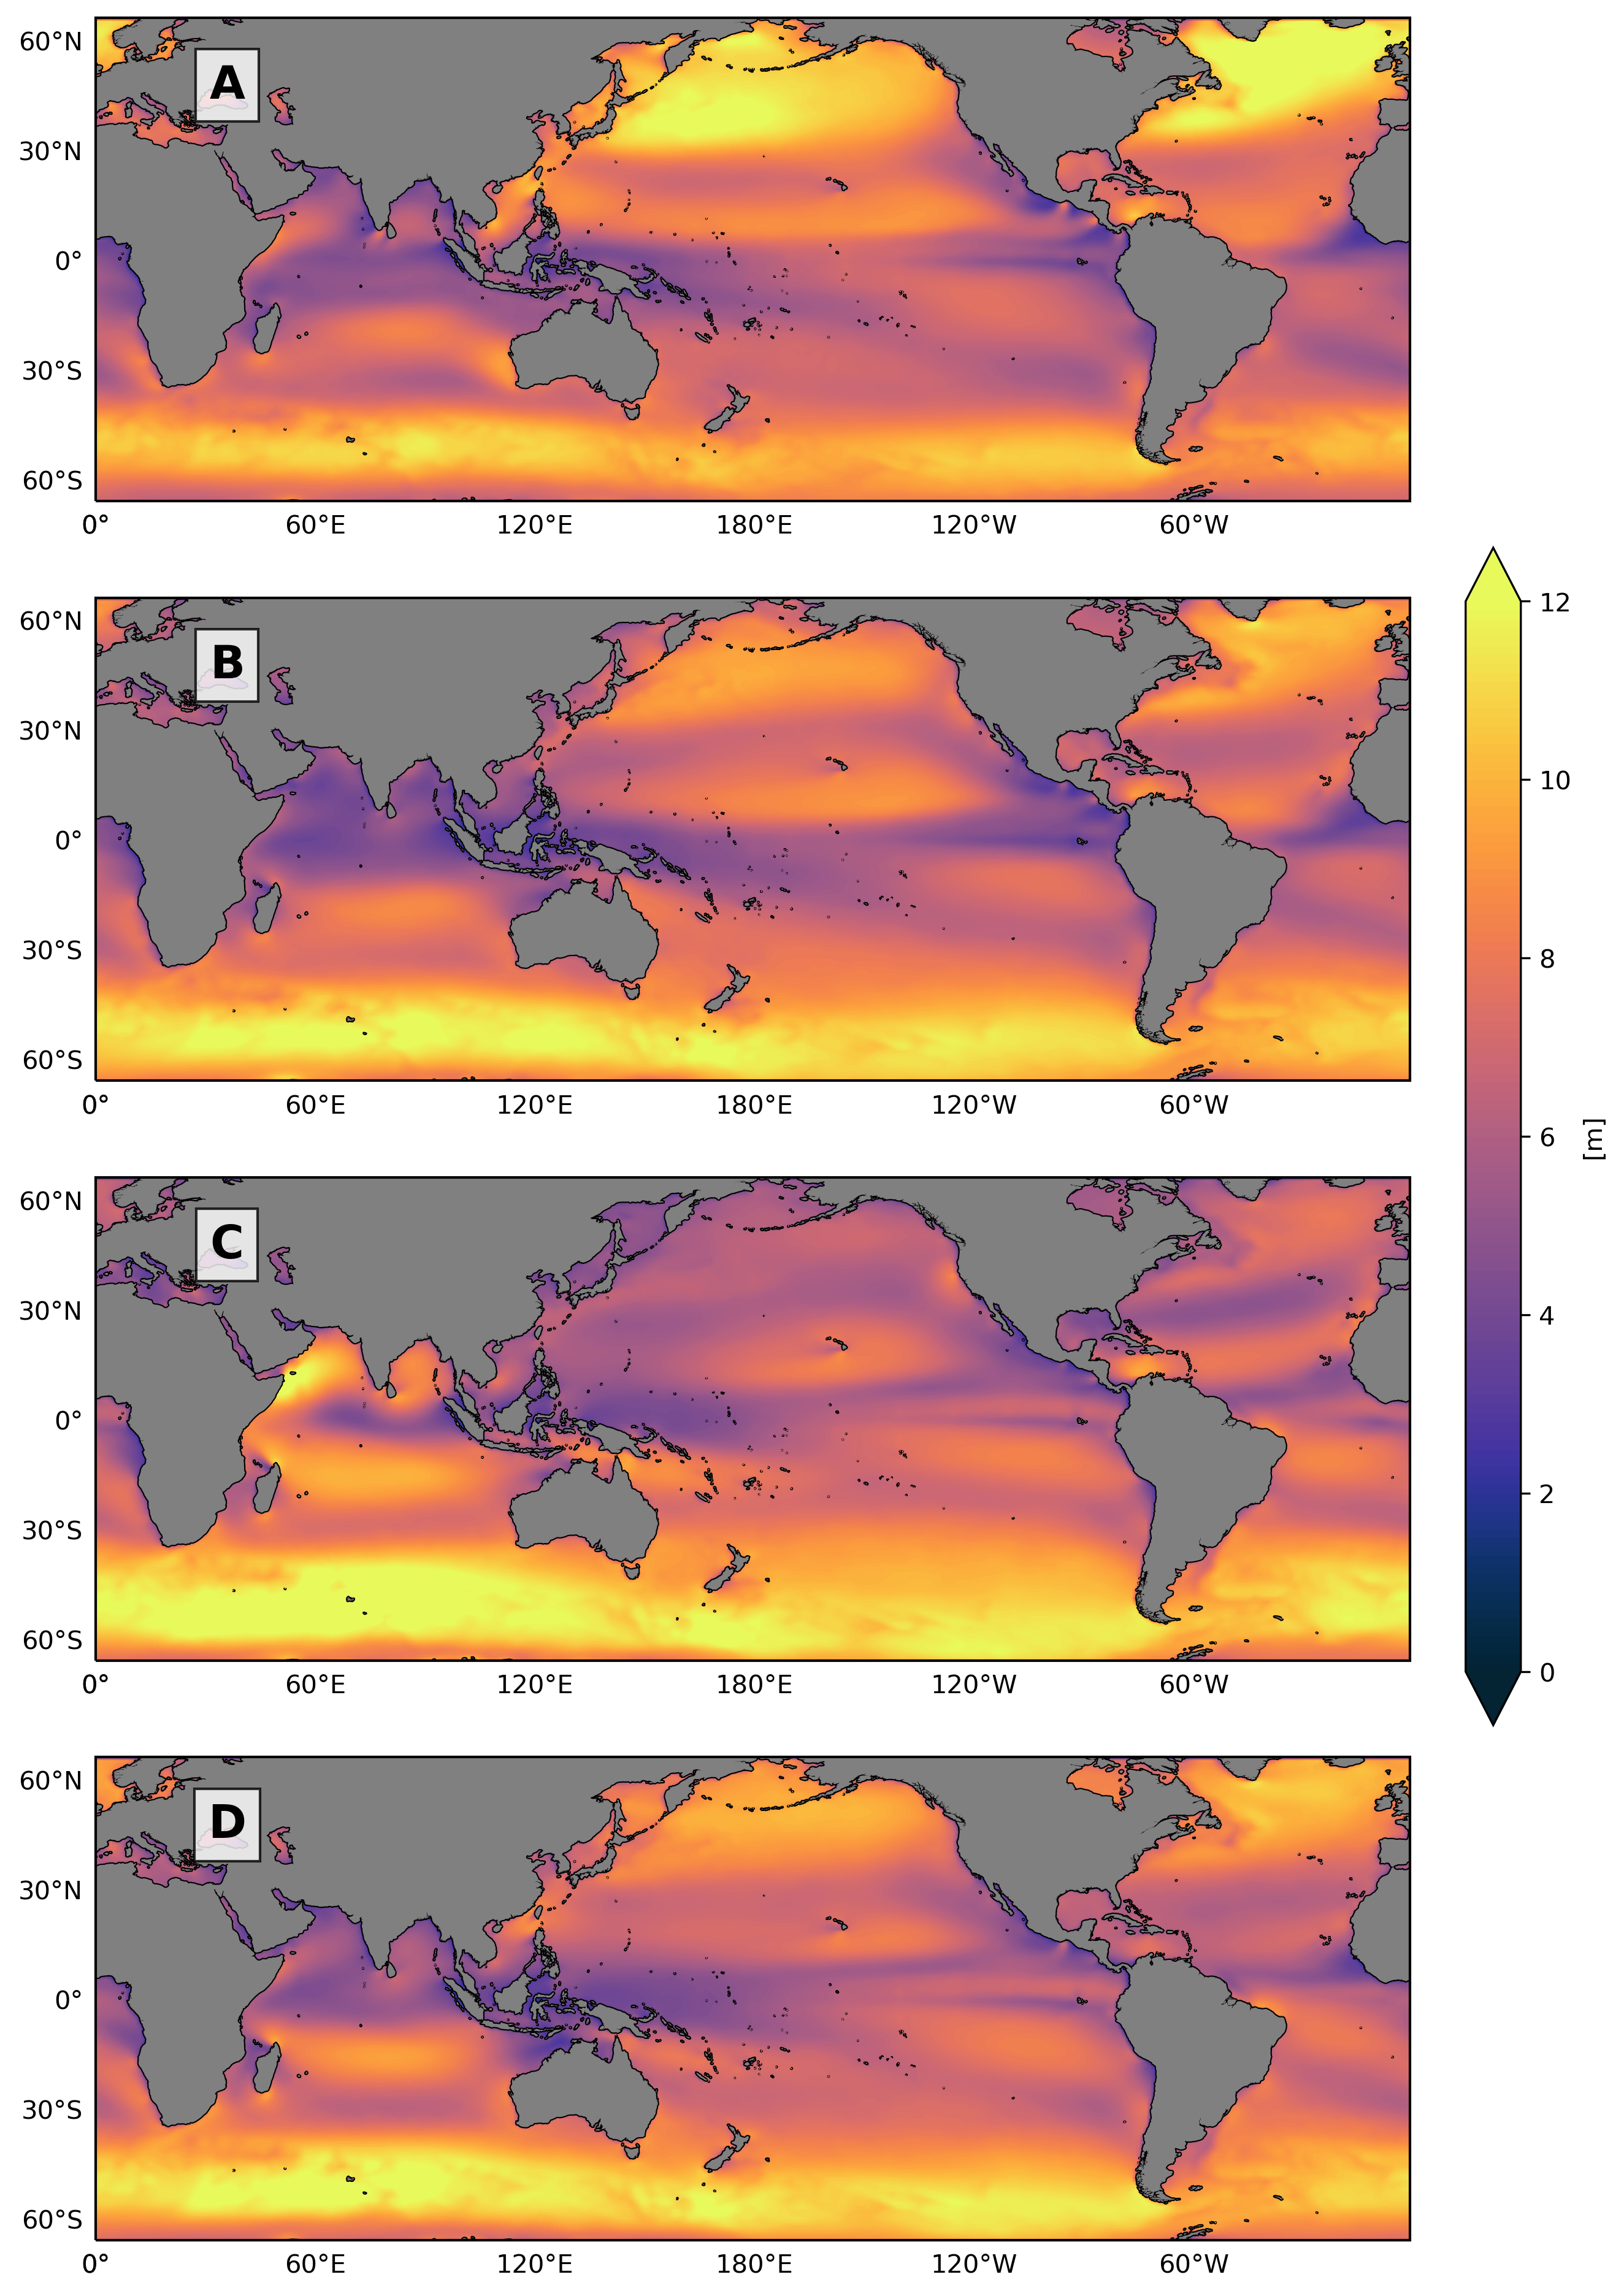
\includegraphics[width=0.5\textwidth]{figs/statistical_moments/CCMP2_seasonal_mean_wsp.png}
    \caption{CCMP2 WSP Seasonal Mean}
    \label{CCMP2_wsp_seasonal_mean}
  \end{minipage}
  %
  \begin{minipage}{.5\textwidth}
    \centering
    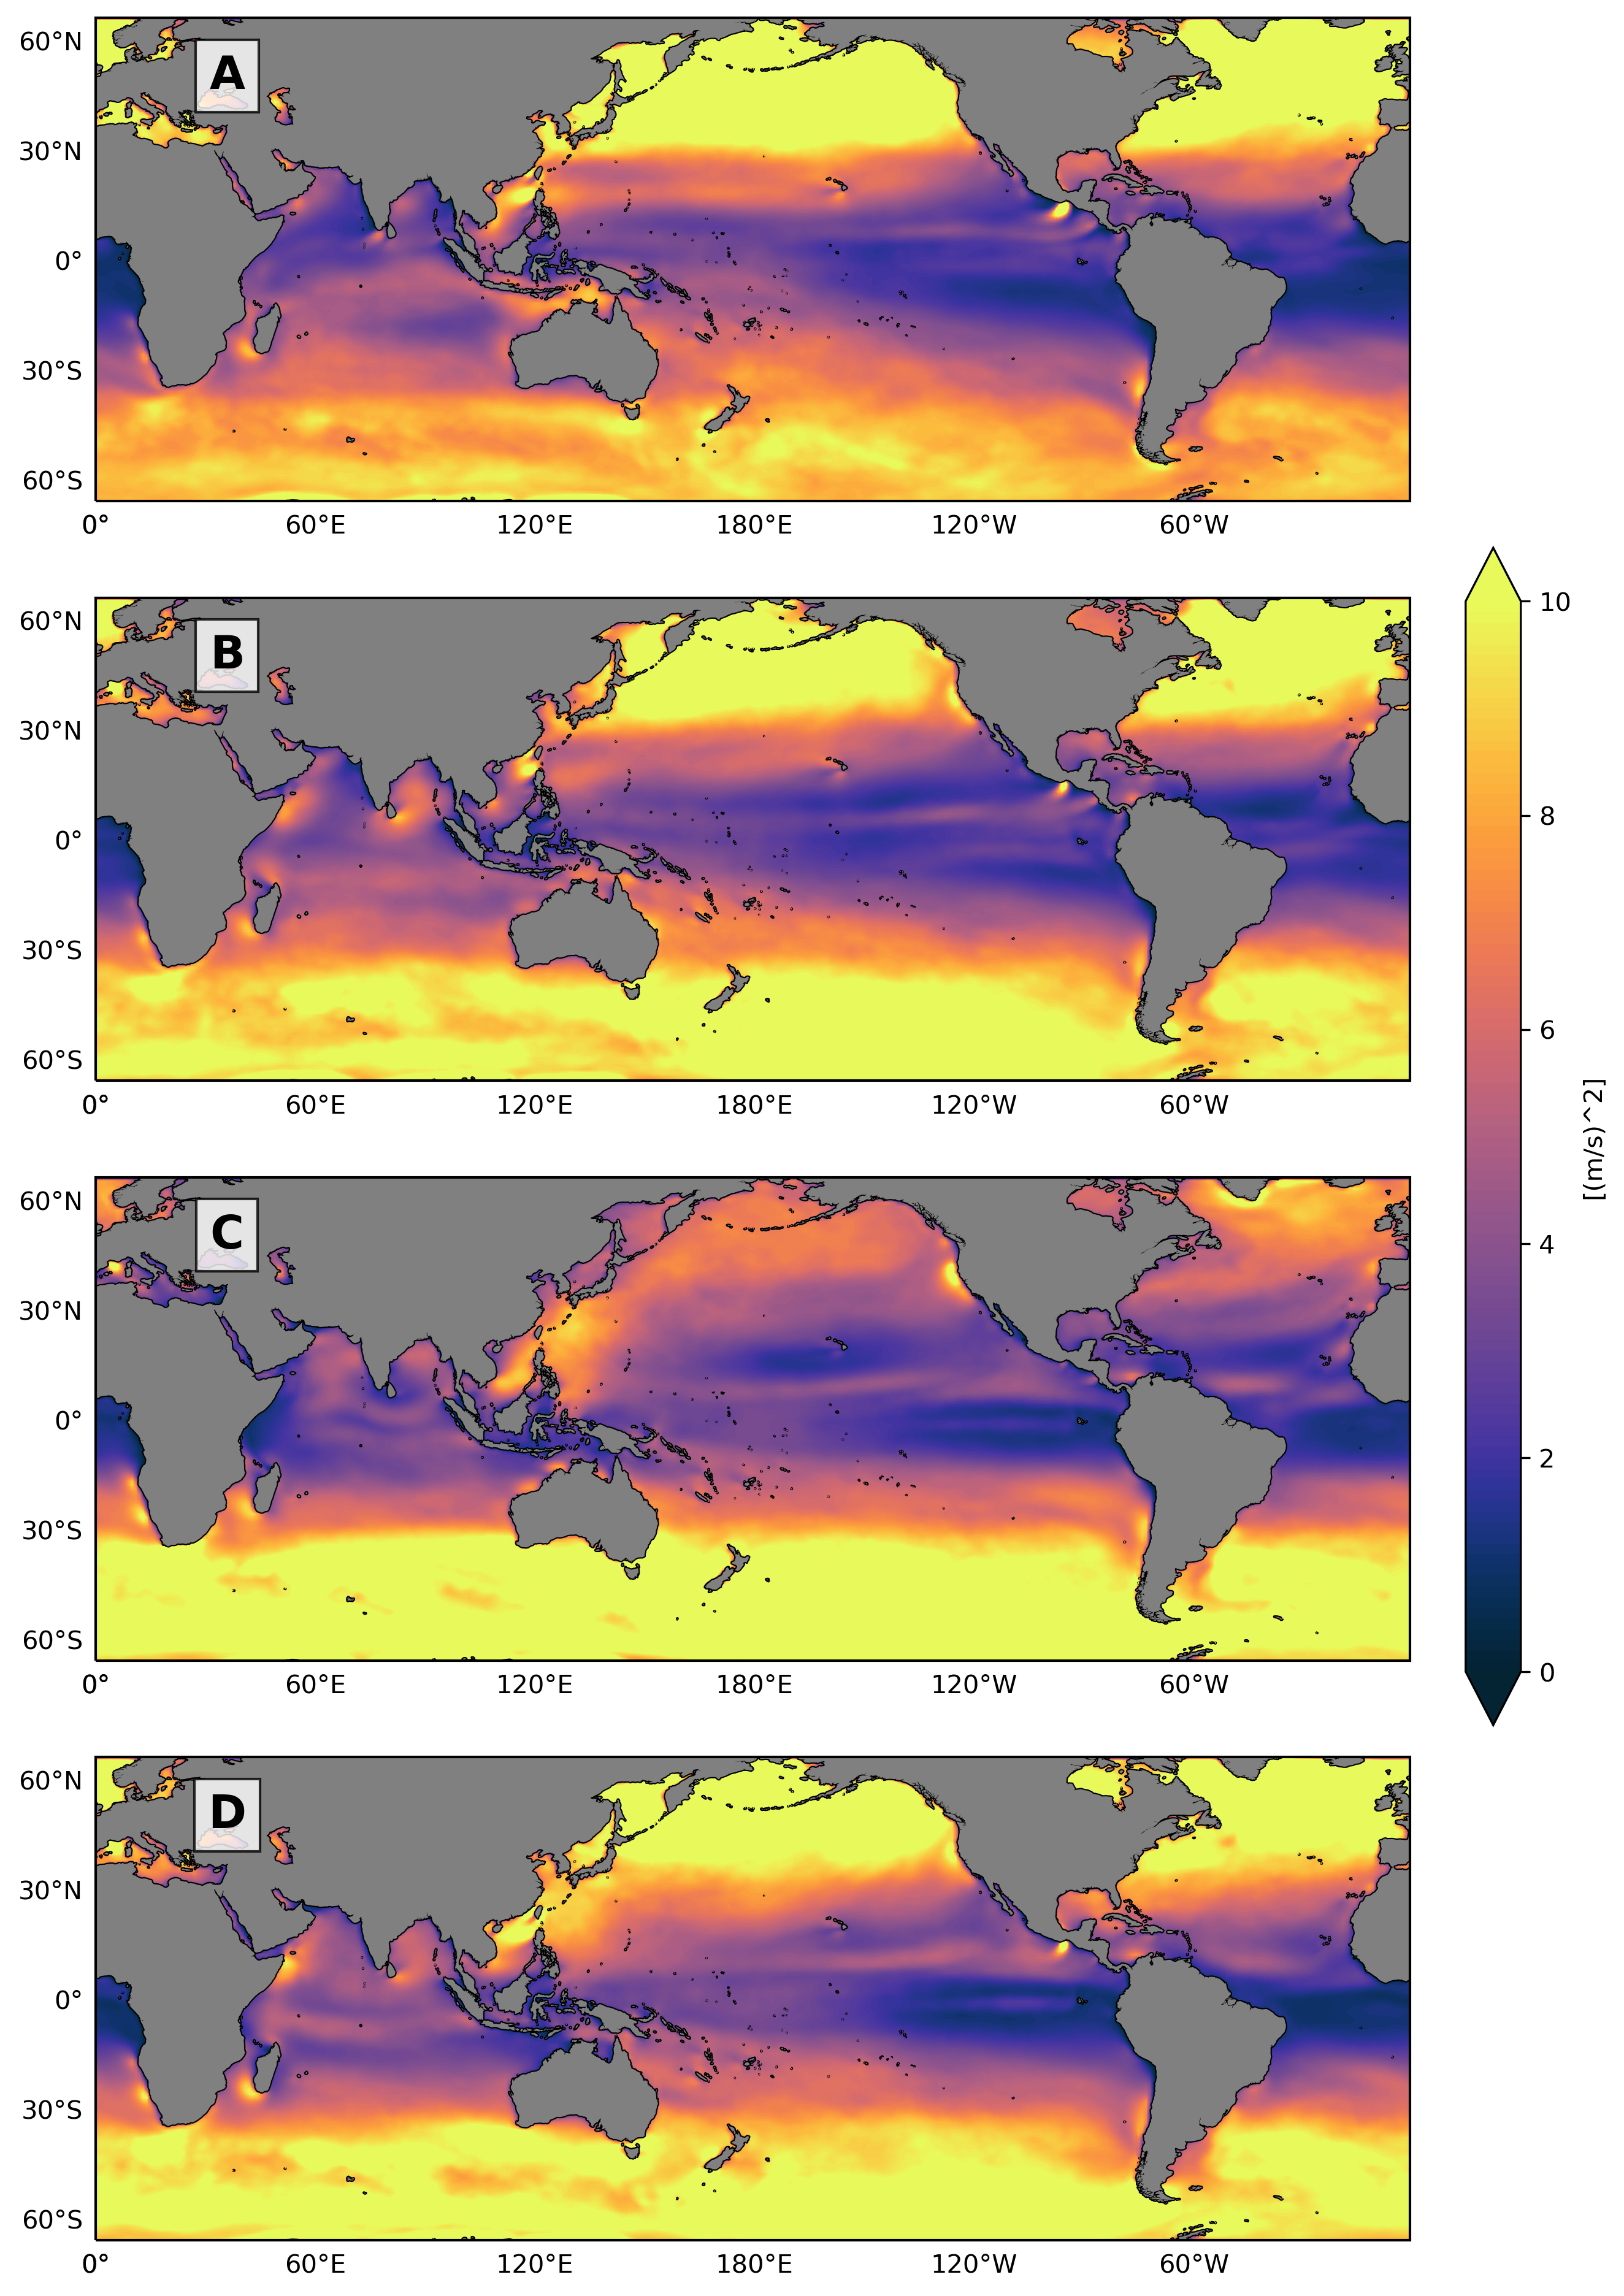
\includegraphics[width=0.5\textwidth]{figs/statistical_moments/CCMP2_seasonal_var_wsp.png}
    \caption{CCMP2 WSP Seasonal Variance}
    \label{CCMP2_wsp_seasonal_var}
  \end{minipage}
%\caption{CCMP2 WSP First and Second Statistical Moments seasonal progression with A) December through February, B) March through May, C) June through August, and D) September through November}
\label{ccmp2_wsp_seasonal_pro}
\end{figure}

The SWH and WSP annual cycle phase maps display an interesting relationship between deviations in the SWH seasonal cycle and local wind anomalies that are generated by similar mechanics to expansion fan wind events off the California coast. In the SWH annual phase constant maps, deviations from the seasonal cycle predominantly cannot be observed in the cases when the deviation in the seasonal cycle is less than the maximum values of the seasonal sinusoidal oscillations. However, this is not the case for all EBRs, as will be explained later.  

For the WSP annual cycle phase map, the phase constant clearly outlines regions where local wind anomalies similar to the expansion fan wind event off the coast of California are present. The wind anomalies are characterized on the phase map by a $\pi$ phase shift in the WSP seasonal cycle from the surrounding region. By looking at the global map of phase constant for WSP, we observe that EBRs typically are out of phase with the surrounding regions. For example, in the EBR off the coast of Australia (Fig~\ref{Ifremer_ccmp2_lsf_chars}F), the phase is approximately 1 radian, while the surrounding regions is between -1.5 and -2 radians. This means that the maximum WSP is reached during the spring and summer months of the Southern Hemisphere within the EBR while the maximum WSP is reached during the winter months of the Southern Hemisphere outside the EBR. 

The WSP phase map has structural similarities to the SWH phase map: the Northern and Southern Hemispheres are $\pi$ out of phase with each other, and the Southern Hemisphere has more spatial variability due again to consistently high variability in WSP in the Southern Hemisphere  (Fig~\ref{CCMP2_wsp_seasonal_var}). However, there are many differences. The phase boundary in the Pacific designating the transition in the hemisphere that is primarily setting the WSP seasonal cycle is further norht, and the majority of the boundary is smooth and continuous, without abrupt changes in phase on the eastern side of the Pacific, but with a slightly high gradient on the west side. In the Atlantic, the phase boundary is a smooth transition and is more linear in shape than the SWH phase boundary in the Atlantic. The phase boundary in the Atlantic follows closely the near zero WSP amplitude of the annual cycle; however, in the Pacific, the amplitude does not tend to zero near or at the equator. Furthermore, the Indian Ocean has prominent structures of swooping fingers of high phase constant values which are difficult to see in the SWH phase map. 

Coefficient of determination global maps can be used to assess the percentage of the variability explained by the model in order to understand whether there are other processes not accounted for by the annual and semi-annual cycles.  Fig~\ref{Ifremer_ccmp2_lsf_gof} shows that the percent of variability explained by the model is high in the North Pacific and Atlantic and low in the Southern Ocean for SWH and WSP. For SWH, the percent variation explained reaches a minimum in the near-equatorial region in the Pacific and Atlantic. For WSP, the features of high percent variation explained are complex throughout the equatorial region with varying amounts from near 100\% to near 0\%. These low values in the equatorial region may be attributed partly to the decadal oscillation of El Ni\~no. The percent variation varies for each EBR. For both SWH and WSP, EBRs range from having 10\% to 40\% of the variation explained by the two modes represented in the model with the exception of the Arabian and Caribbean seas which have near 100\% variation explained. There are especially low values off the coast of Chile and Namibia for SWH and off the coasts of California, Chile, and North Africa for WSP. The Arabian and South Caribbean seas have higher percent variation explained by the model because these regions primarily have wave and wind forced by mechanics that have annual and semi-annual frequencies. In support of this argument, both of the coefficient of determinations geographic features follow very closely with geographic features in the annual and semi-annual amplitude of SWH and WSP maps such that the percent of variation explained by the model is highest in regions with high amplitude and lowest in region of near zero amplitude. This means that the model explains the variability significantly less in most of the EBRs because there are  weak annual and semi-annual cycles. In addition, there are other forcing mechanism at work in these regions that contribute more significantly to the wave and wind field. One of these forcing mechanisms for the wave field is the deviation from the seasonal cycle from local wind events. The goodness of fit quantified by the coefficient of determination should not be thought of as a test of reliability of the model. Rather, it is an indication of physical processes not accounted for by the model, which we want to explore to understand the underlying mechanisms generating the variability in the wave and wind fields. 

\begin{figure}[tbh]
\centering
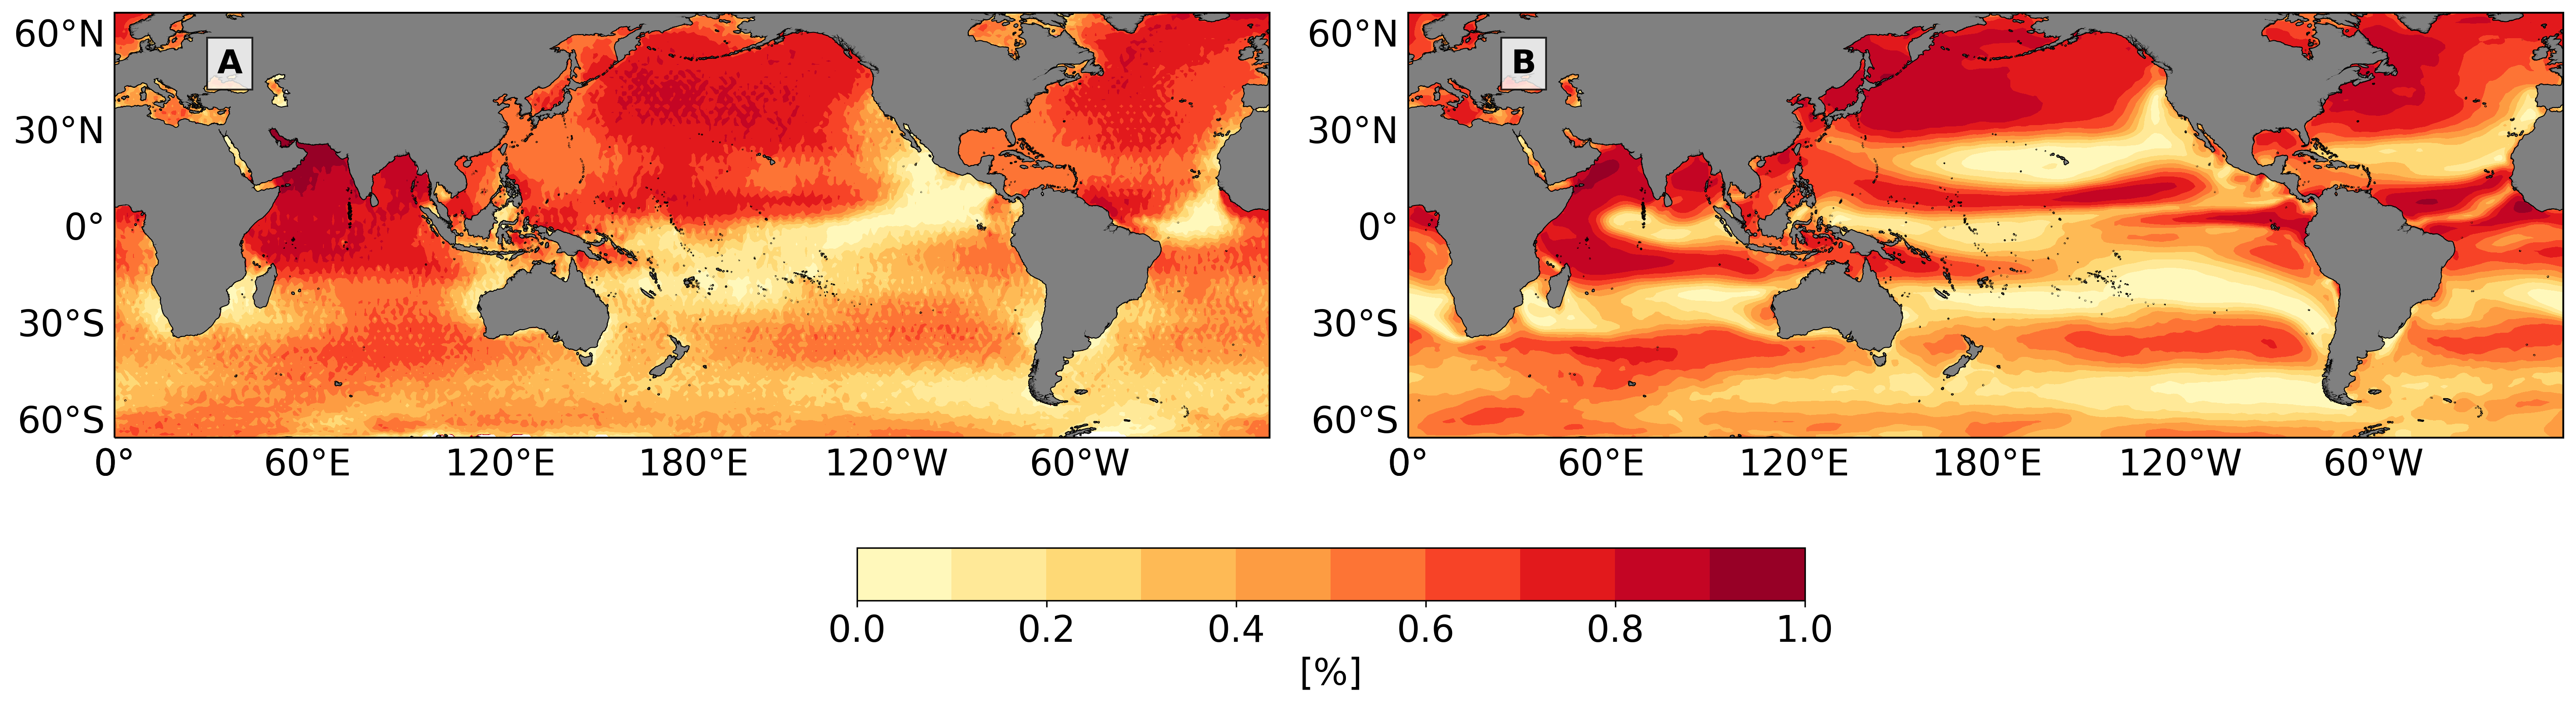
\includegraphics[width=1.0\textwidth]{figs/lsf_characteristics/ccmp2_ifremer_goodness_of_fit_5_par.png}
\caption{Global map of Coefficient of determination for Ifremer SWH (A) and CCMP2 WSP (B) using Unweighted Annual and semi-annual Least Square Fit from January 1st, 1993 to December 31st, 2015 for a metric of the goodness of fit of the model.}
\label{Ifremer_ccmp2_lsf_gof}
\end{figure}

\subsection{Regional Climatologies of EBRs}

In order to obtain a closer look at the seasonal cycle within these EBRs, climatologies or monthly mean SWH and WSP time series were computed from January 1st, 1993 to December 31st, 2015 within 4$^{\circ}$ by 4$^{\circ}$ grid boxes. Fig~\ref{reg_clima_nh} and Fig~\ref{reg_clima_sh} show the regional climatologies from EBRs in the Northern and Southern Hemispheres respectively as well as the 4$^{\circ}$ by 4$^{\circ}$ regions within each EBRs where the climatology is computed. From these climatologies, a consistent trend is seen. In all EBRs, the maximum in the WSP seasonal cycle occurs at the same time, when a deviation from the sinusoidal SWH seasonal cycle occurs. 

\begin{figure}[tbh]
\centering
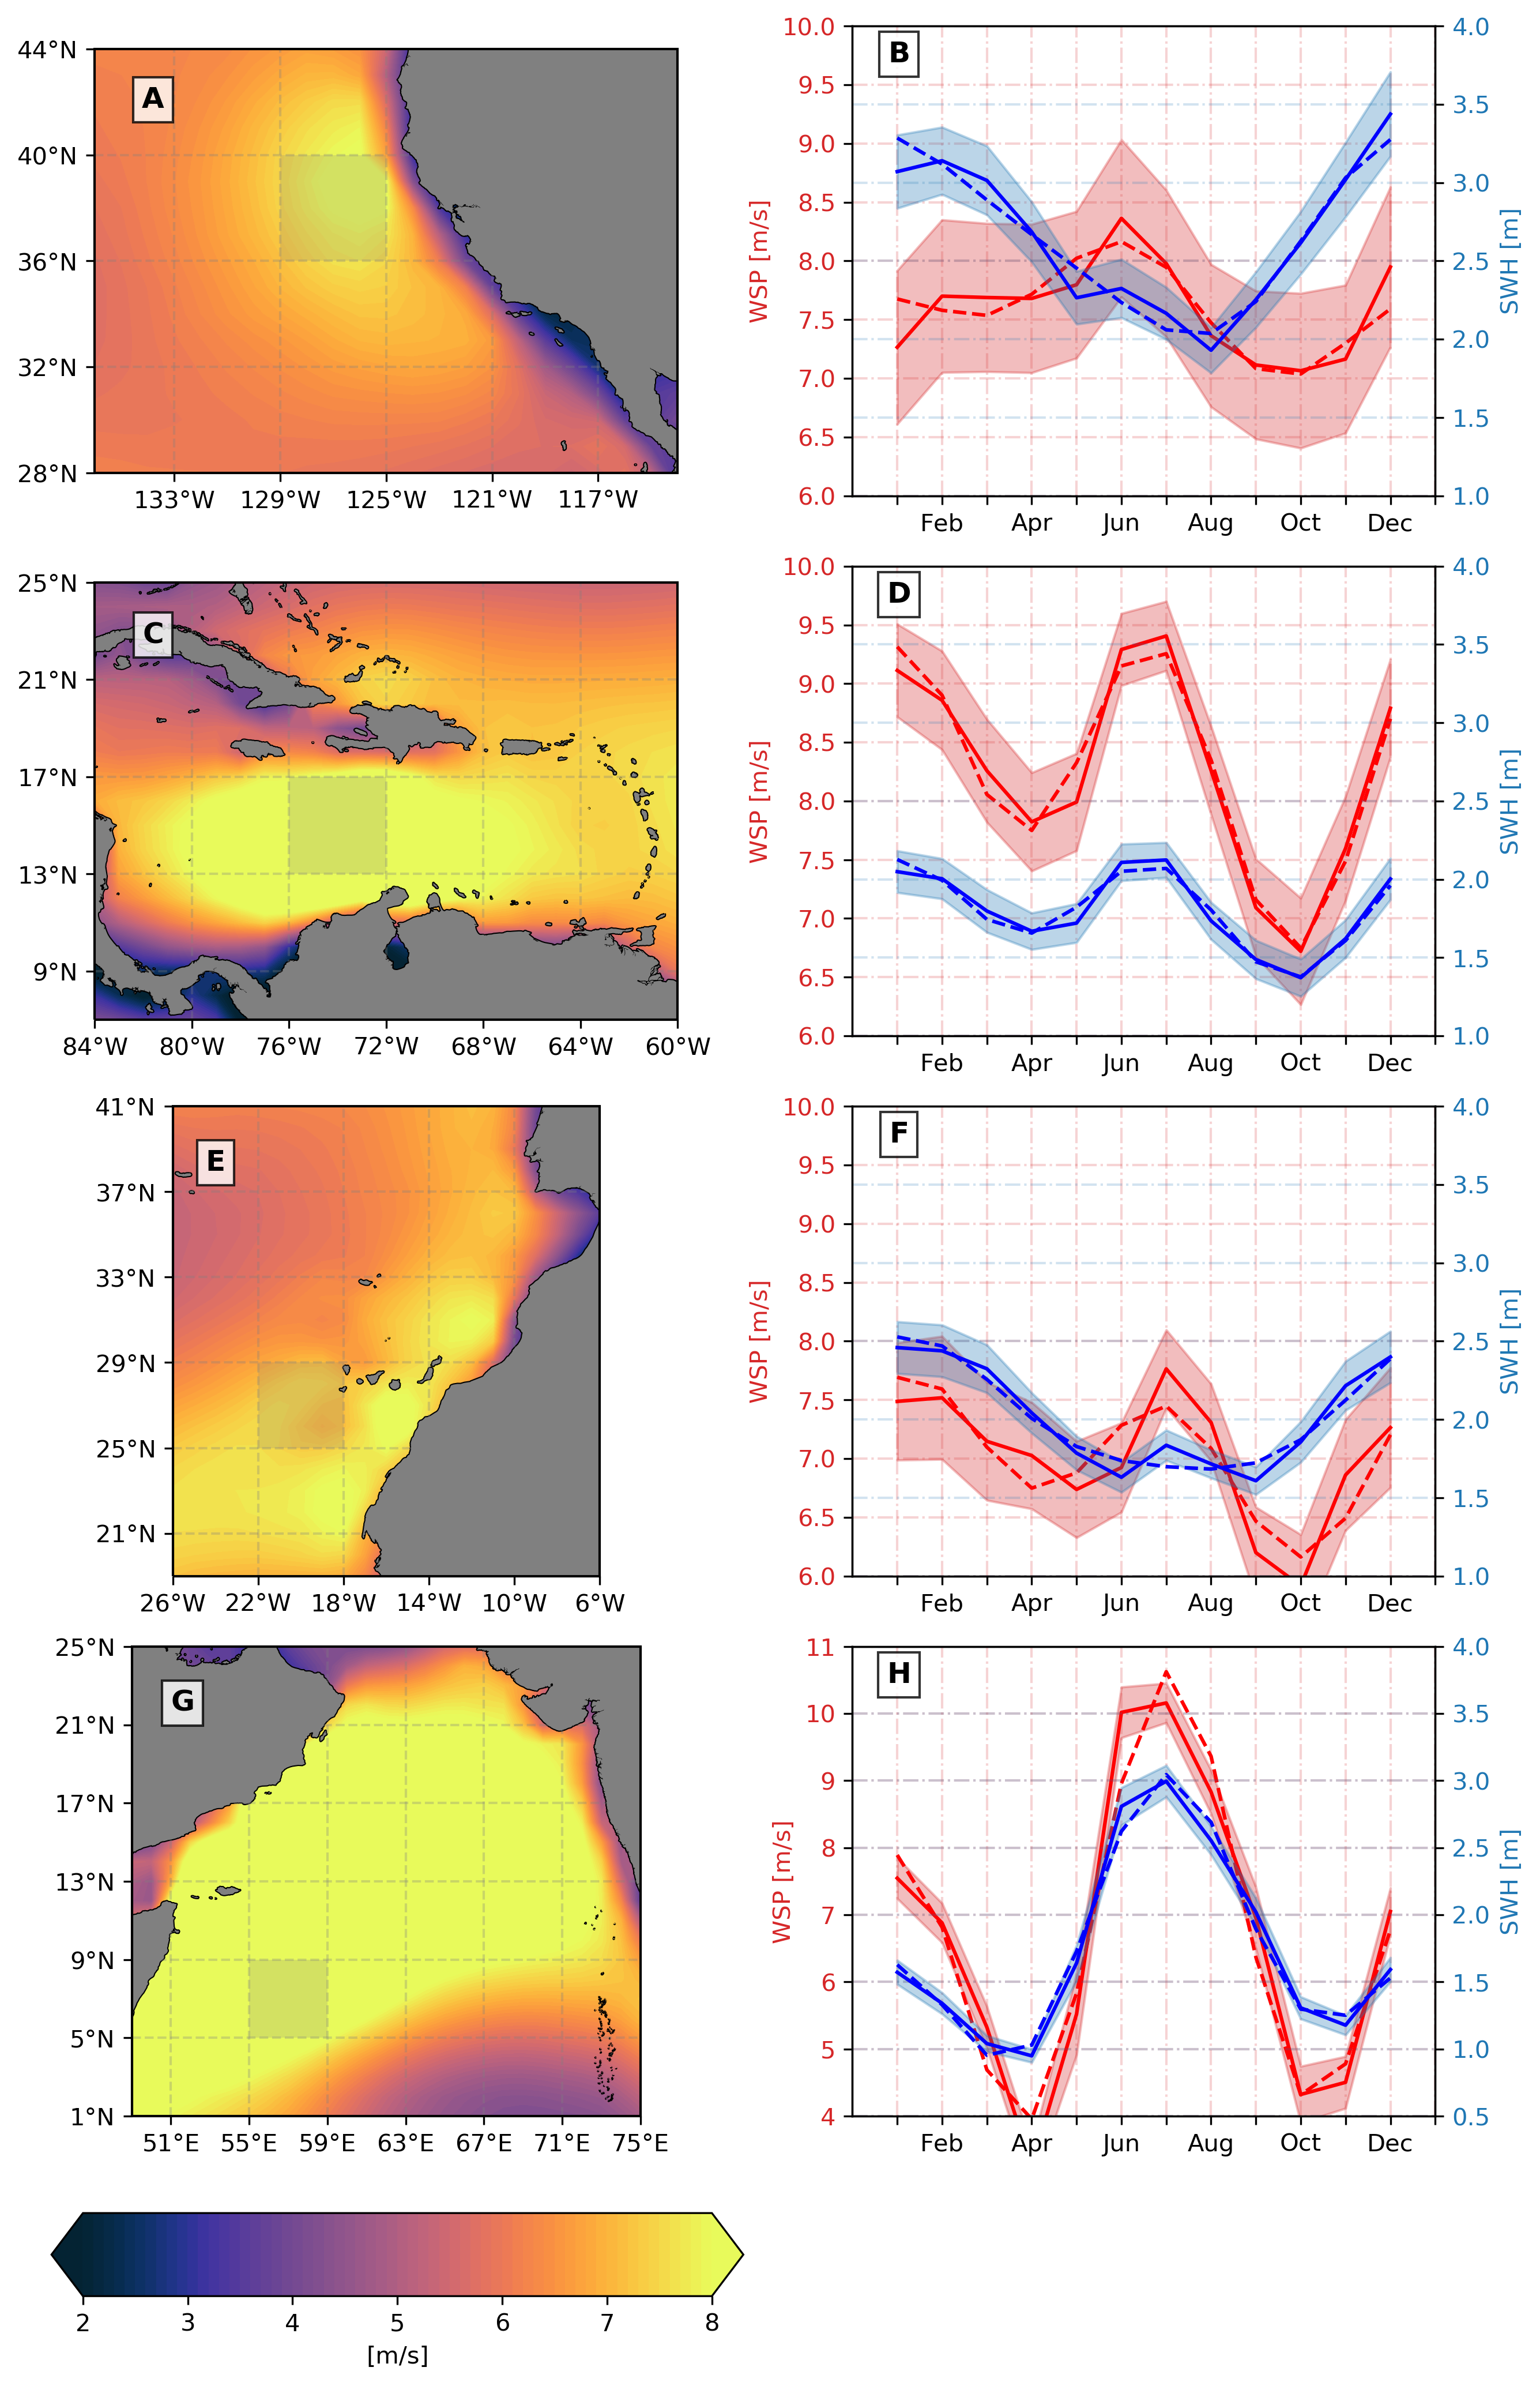
\includegraphics[width=0.5\textwidth]{figs/regional_climatologies/paper_regional_clima_nh.png}
\caption{EBR regional maps of WSP averaged over the months of June, July, and August (left column) with Ifremer SWH (solid blue curve) and CCMP2 WSP (solid red curve) climatologies in shaded 4$^{\circ}$ by 4$^{\circ}$ boxes within EBRs located in the Northern Hemisphere. Shading in climatologies represents the standard error of the mean and dotted blue and red lines are the annual plus semi-annual cycle least-squares fitted to monthly climatology for SWH and WSP respectively. EBRs include Northern California (A and B), Southern Caribbean Sea (C and D), North Africa near the coast of Morocco and western Sahara (E and F), North-Western Arabian Sea (G and H) }
\label{reg_clima_nh}
\end{figure}

\begin{figure}[tbh]
\centering
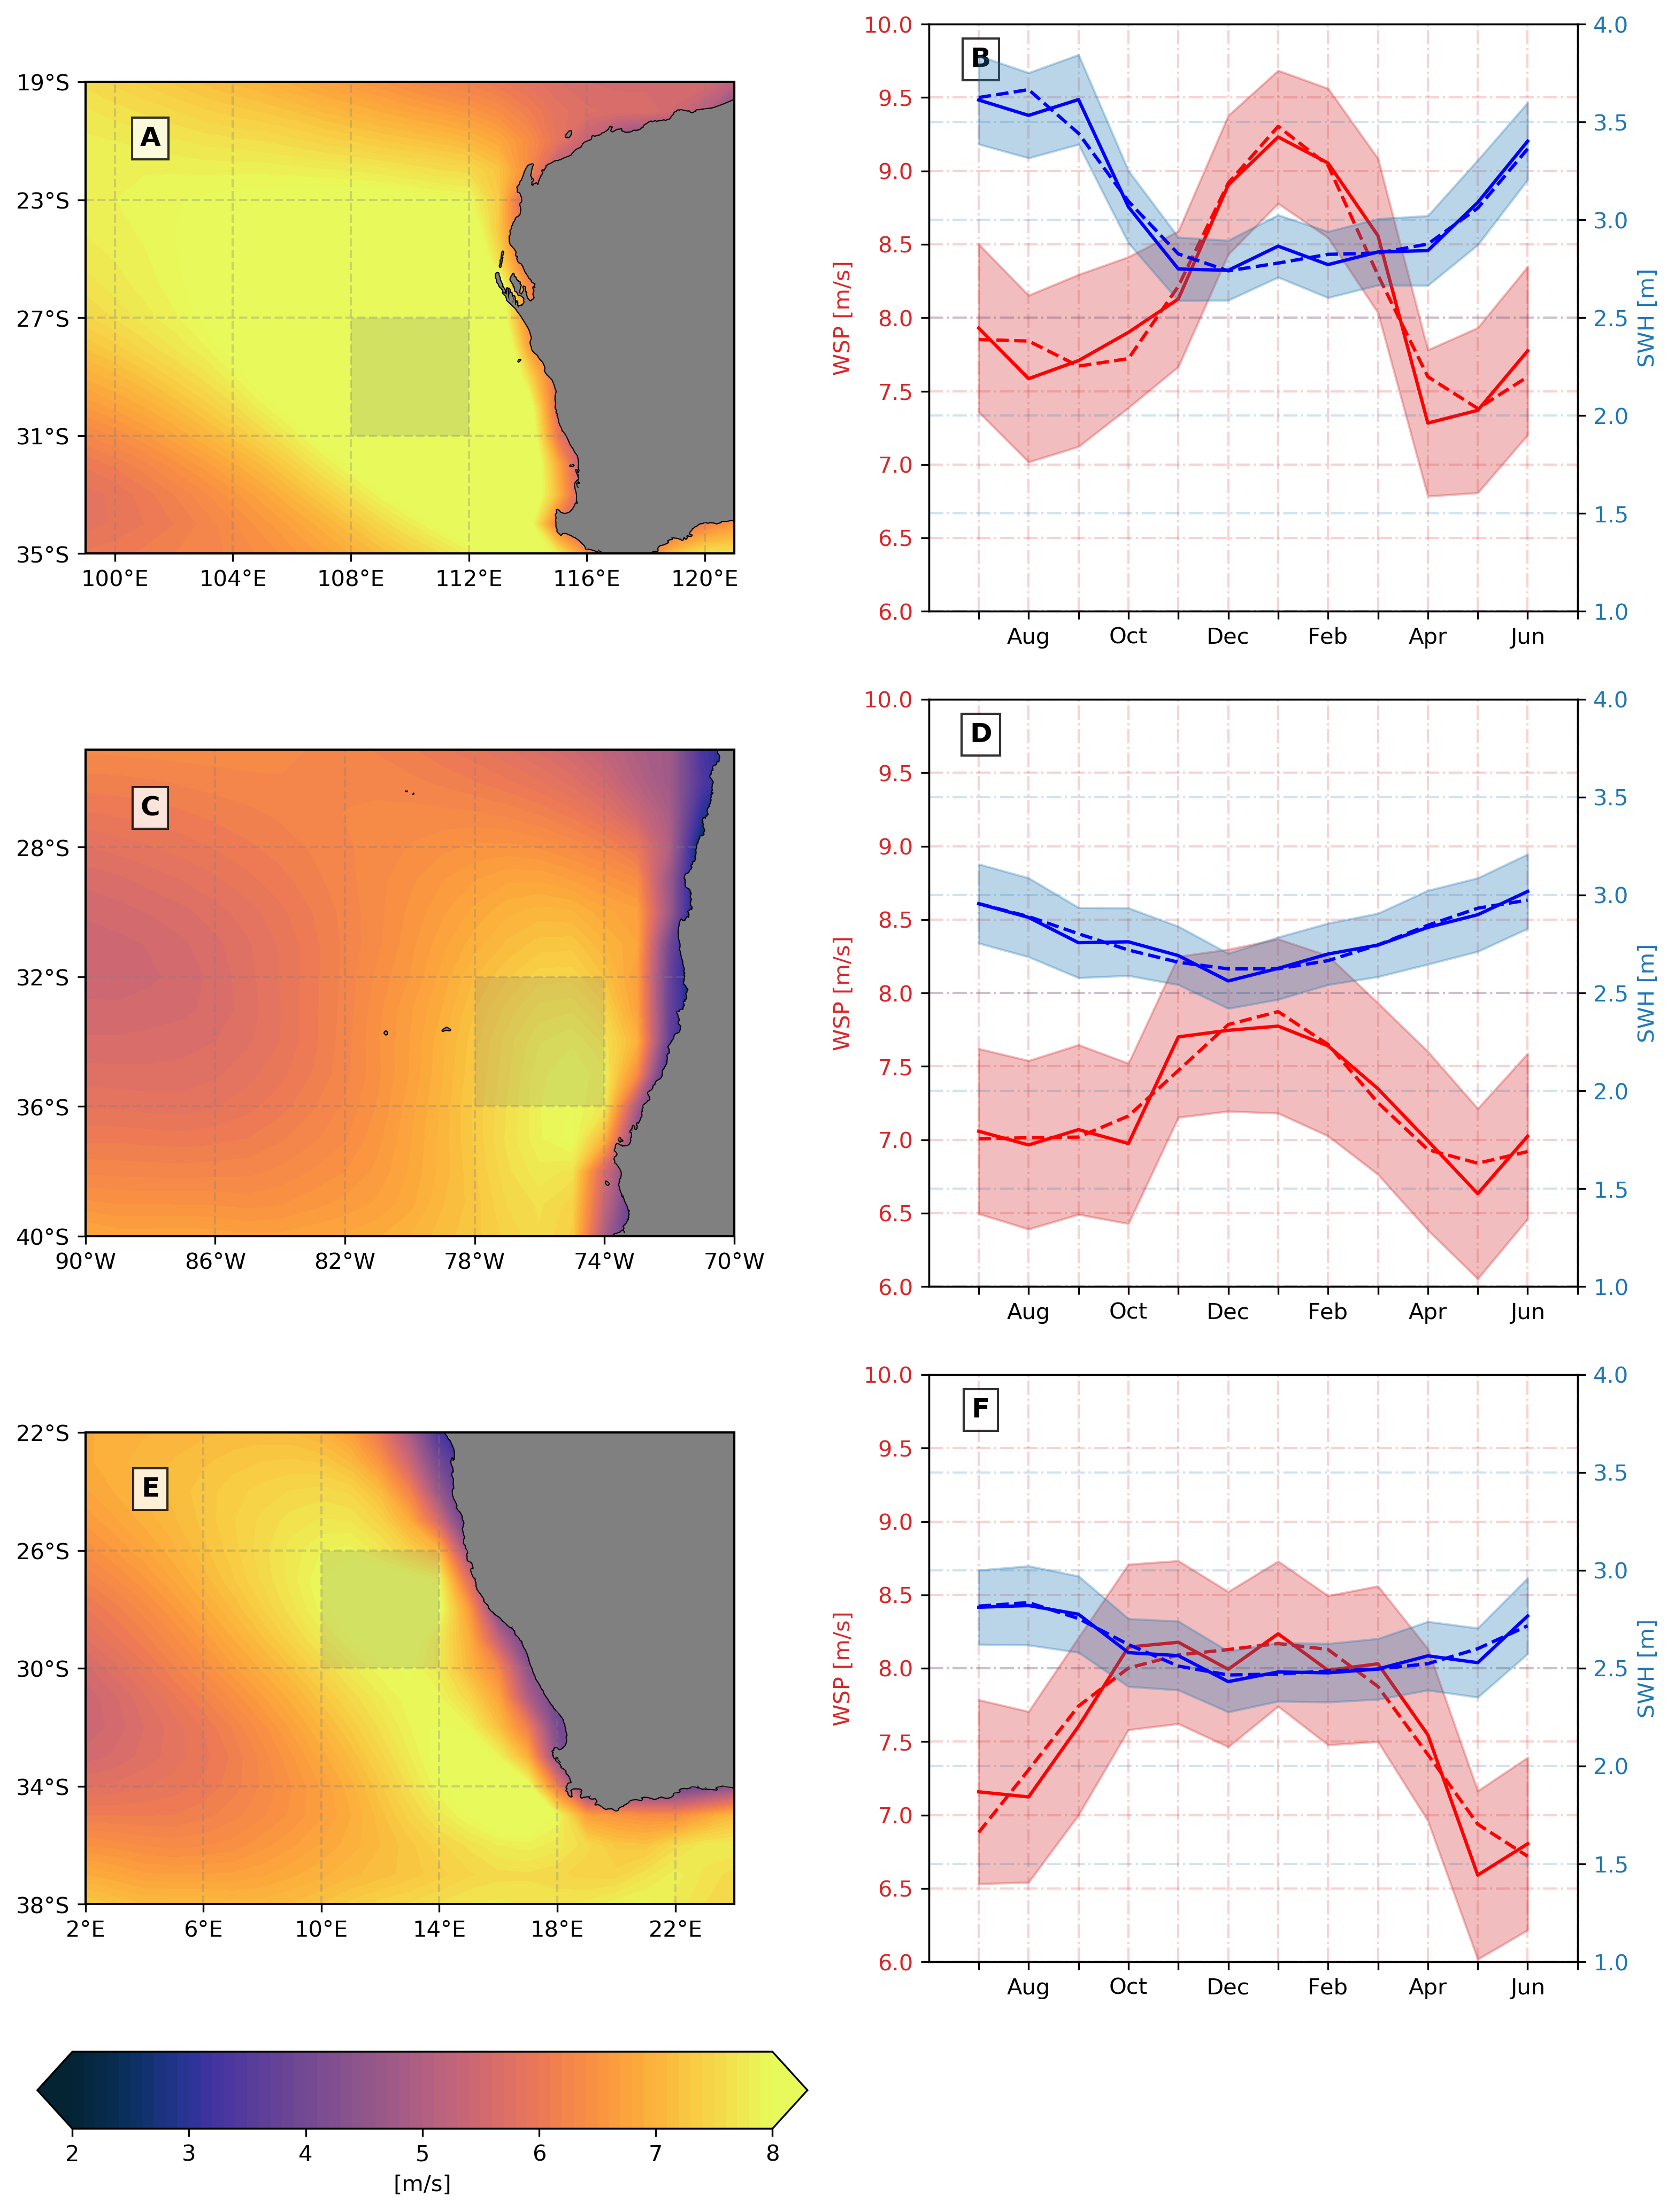
\includegraphics[width=0.5\textwidth]{figs/regional_climatologies/paper_regional_clima_sh.png}
\caption{EBR regional maps of WSP averaged over the months of December, January, and Feburary (left column) with Ifremer SWH (solid blue curve) and CCMP2 WSP (solid red curve) climatologies in shaded 4$^{\circ}$ by 4$^{\circ}$ boxes within EBRs located in the Southern Hemisphere. Shading and dotted lines are as in Fig.~\ref{reg_clima_nh}. EBRs include Western Australia (A and B), Central Western coast of South America near Chile (C and D), and South-Western Coast of Africa near Namibia (E and F)}
\label{reg_clima_sh}
\end{figure}


%In addition, by computing the residual at each time step between the same 5 parameter least square fit model used in the global analysis, it was observed that the residue values in EBRs during the month of the local wind anomaly's presence had significantly larger than other residue values in the rest of the time series. However, this was not true for all EBRs. Those EBRs in monsoon regions with high magnitude deviations comparable to maximum of the seasonal cycle had lower residual values.

Examples include the Northern California and North African EBRs. Off the coast California, the WSP seasonal cycle reaches a maximum during the month of June. This peak is associated with an increase in SWH at the same time that the seasonal cycle is reaching a summer minimum. In the North African region off the coast of Morrocco, a WSP maximum and a deviation from the SWH seasonal cycle are present in the month of July. Even though deviation seem to be present in all climatological maps, the magnitude and significance of the deviation varies from region to region. 

The magnitude of the deviation in the SWH cycle is determined by the local conditions and characteristics of the wave field within the region. Local conditions refers to the exposure and distance of the EBR from remotely forced waves generation regions. In other words, how close the EBR is to regions with storms that produce high SWH remotely forced waves. For example, in the southern Caribbean Sea, the SWH  seasonal cycle is in phase with the WSP seasonal cycle in Fig~\ref{reg_clima_nh}D. This is consistent with the hypothesis that local wind events, including the wind anomaly during boreal spring, generate the waves within the region. Waves within this region have little exposure to waves propagating from the high latitudes of the northern or southern Atlantic and little of the wave energy is remotely forced.  This shelter from remotely forced waves is due to the Caribbean islands that ring the Caribbean sea (Fig~\ref{reg_clima_nh}C). In this example, the deviation from the seasonal cycle is substantial such that the deviation is of similar or equal magnitude to the maximum of the annual cycle. Therefore, the local wind anomaly significantly alters the seasonal cycle of SWH causing two maxima in SWH per year. This explains the near out of phase values seen in the Caribbean sea with respect to the rest of the Northern Hemisphere  (Fig~\ref{Ifremer_ccmp2_lsf_chars}E). In addition, in Fig~\ref{Ifremer_ccmp2_lsf_chars}C,D, the large semi-annual cycle in the SWH and WSP semi-annual amplitude maps is clearly seen in the South Caribbean Sea due to the local wind anomaly. This same semi-annual pattern occurs in the Arabian and South China seas, where monsoon winds generate high locally forced waves, creating a significant deviation from the annual cycle.   

On the western coast of Australia (Fig~\ref{reg_clima_sh}B), the EBR is exposed to the Southern Ocean where larger storms produce larger SWH remotely forced waves. These waves propagating into the EBR cause there to be a high mean SWH which the SWH seasonal cycle oscillates about. This larger SWH mean overpowers the SWH signal generated from the local wind anomaly such that the magnitude of the deviation from the seasonal cycle is less than other EBRs. This same effect occurs in the two other Southern Hemisphere EBRs. Off the coast of Chile and Namibia (Fig~\ref{reg_clima_sh}D,F), deviations from the seasonal cycle occur in November and are hardly noticeable. These deviations line up with a maximum in the WSP climatology.

The significance of deviation from the seasonal cycle can be determined by considering the standard error of the mean (Figs.~\ref{reg_clima_nh},\ref{reg_clima_sh}). In regions with high variance, the standard error of the mean is large enough that the deviation from the seasonal cycle is not statistically significant. This is seen in the west coast of Australia, coast of Chile, and the coast of Namibia.  

%possible look at the Chi-square value at time step such that we normalize the residue (model - data) by the standard error of the mean in order to determine statistical significance of deviation. By normalizing the residue with the standard error of the mean at each time step, a chi-square statistic can be obtained to determine which deviations from the seasonal cycle are statistically significant.


\section{Discussion}

\subsection{Local vs. Remotely Forced Waves}

In order to evaluate whether EBR waves are generated by local wind events, we use wave age information to classify waves as locally or remotely forced. During a storm, wind blows over a length of ocean surface called fetch at certain speed and for a given time duration, generating a packet of waves. Initially, waves that are formed by the wind are categorized as locally forced waves since the atmosphere is still supplying energy and momentum to the waves. These local forced waves are commonly called wind-seas. The frequency or wavenumber spectrum is evolving as wave height, frequency, and period of the waves grow. These waves tend to have shorter periods (or high frequency and wavenumber) and thus travel at slower phase speeds than long period waves. Once the wind is no longer inputting energy and momentum into the waves, the waves are categorized as remotely forced waves. Remotely forced waves are commonly called fully developed seas or swell. In the case of swell waves, the wave field's frequency or wavenumber spectrum is set and is no longer evolving. These waves tend to have long periods (or low wave frequency and wavenumber) and have the ability to traverse long distances at higher phase speeds than short period waves. This leads to the dispersive nature of deep water surface gravity waves \cite{snodgrass1966propagation}. \citet{ardhuin2009observation} observed swells propagating across ocean basins using satellite altimetry data from ENVISAT and showed that steep swell waves lose a significant fraction of there energy (up to 68\%) over distances of 2800 km due to the laminar to turbulent transition in the air-side boundary layer. Wind-sea waves tend to be steep because of their short periods and high amplitudes, and this leads to significant dissipation over relatively short distances. In addition, wind-sea dissipation could also be due to small scale wave-wave interactions, wave-current interactions and other atmospheric forcing. Therefore, the wind event must be relatively in close proximity to wind-sea waves.  

Waves measured by satellite altimeters represent a superposition of local wind waves and remotely generated swell, and the altimeter does not distinguish frequency, period, or direction.  The sea surface backscatter power received  by the satellite altimeter averages over all wave of varying wave height, frequency, and direction present in the satellites footprint \cite{fu2000satellite}. 

%However, the dominant wave height within the satellite's footprint is only recorded. Therefore, local wind events have varying degrees of influence on the annual cycle of swh depending on the amount of remotely forced waves that enter a given region. 

Globally, the wave field is consistently dominated by swell \cite{chen2002global,semedo2011global}. \citet{chen2002global} used collocated satellite altimetry SWH and radiometer WSP from the Jason-1 satellite mission to compute the probability of swell using a wind-wave relationship derived from WAM wave model which was able to separate wind-seas from swell. Global seasonal maps of probability of swell showed that the SWH observations by satellite altimetry are categorized primarily as remotely forced waves in all oceans with lower probability of swell in the Southern Ocean, in coastal regions, and along common storms tracks \cite{chen2002global}. The probability of swell also undergoes a seasonal cycle with a decreasing amplitude going from high to low latitude. This decrease in probability of swell indicates an increase in the amount of wind events generating wind seas that dominate the wave field. \citet{semedo2011global} built on this analysis, using wave energy spectra from WW3 ECMWF to first compute SWH, mean wave period (MWP) and mean wave direction (MWD) and then separating SWH, MWP, and MWD into wind-sea and swell components using WAM separation frequencies. From seasonal maps of SWH decomposed into swell and wind sea components, the swell SWH component was found to be always higher than the wind-sea component implying that swell accounts for the majority of the SWH signal. In addition, probability of swell was compute using wave age which again showed swell dominating the wave field \cite{semedo2011global}. In the probability of swell maps, similar to \citet{chen2002global}, they found high probability of swell consistently throughout the world oceans. In addition, using the directional spectrum, \citet{echevarria2019seasonal} was able to categorize the wave field into five main wave modes for the first empirical orthogonal function in their principal component analysis. This illustrated unimodal variability in the high latitudes with multi-modal in the equatorial region. Each of these modes have been associated with different wind systems that generate these wind waves. In all multi-modal regions, all these modes overlap and coexist with each other to for the seasonal variability of the wave climate \cite{echevarria2019seasonal}.

\subsection{Probability of Swell: Wave Age Method}

In order to confirm that waves observed during the spring months in EBRs were locally forced by local wind anomaly events rather than remotely forced by distant storms, we implemented the \citet{semedo2011global} method of using wave age to compute global probability of swell maps. Wave age quantifies the stage of development of waves and is therefore used to separate locally forced waves from remotely forced waves through an empirically determined criterion. The wave age criterion is defined as 
\begin{equation}
     \mbox{\rm Wave Age} = \frac{C_{p}}{U_{10}},
 \end{equation}
where $C_{p}$ is phase speed of the surface gravity wave or the speed of an individual crest of a wave and $U_{10}$ is the wind speed 10 meters above the ocean surface. The separation value used in our analysis to distinguish locally and remotely forced waves is 
\begin{eqnarray}
     \frac{C_{p}}{U_{10}} & > & 1.2\quad {\mbox{\rm Remotely Forced Waves}} \\
     \frac{C_{p}}{U_{10}} & \leq & 1.2\quad {\mbox{\rm Locally Forced Waves}}
\end{eqnarray}
This criterion is chosen because it has been shown that wave growth stops or at least becomes very slow when wave age is greater than 1.2. This corresponds with waves crests travelling 20\% faster than the wind speed 10 meters above the ocean surface, so that the waves are outrunning the wind and not able to receive further wind energy input.  In order to calculate phase speed of waves, we used Wave Watch 3 (WW3) modeled data with peak frequency. We assume that the the satellite observes deep water waves, with a wavelength much less than the water depth.  For deep water waves, the deep water dispersion relationship yields a peak phase speed : 
\begin{equation}
    C_{p} = \frac{g}{2\pi f_{p}}
\end{equation}

We computed wave age using the WW3 Climate Forecast System Reanalysis data product (CFSR) product, with modelled WSP and peak frequency at 6 hourly temporal and 0.5 degree spatial resolution. The WW3 CFSR product was used instead of the WW3 European Centre for Medium-Range Weather Forecasts (ECMWF) product because CFSR has more seasonal variability, and prediction accuracy improves in recent years \cite{stopa2014intercomparison}. However, the WW3 CFSR data set has some potential biases, including overestimation of SWH and WSP as compared to in situ buoy observations and less temporal homogeneity which manifests itself as a slightly less smooth time series \cite{stopa2014intercomparison}. CFSR more accurately models extreme weather events and detailed processes while ECMWF is more temporally homogeneous \cite{stopa2014intercomparison}. 

%In order to validate that the modelled WW3 CFSR data agrees with observation made by the Ifremer satellite altimetry SWH product and CCMP version 2 WSP product, the WW3 SWH and WSP climatologies are computed and overlaid on the Ifremer SWH and CCMP2 WSP climatology maps. In addition, global maps of swh and wsp characteristics of the 5 parameter least square fit are computed. Visually, it is observed that there is relatively good agreement with the the seasonal cycle monthly mean values between WW3 and Ifremer and CCMP2 data. Notice that there comparisons are performed after significant temporal and spatial averaging. Therefore, this is not a statement for the actual point by point agreement of modelled data versus active remote sensing measurements. Averaging has reduced some of the variability and uncertainty within the two data set which has allowed for the comparison to be viable.

Before computing wave age with WW3, we visually compared WW3 SWH and WSP and Ifremer SWH with CCMP2 WSP least square fit characteristics and regional climatologies to make sure that the model was representing the data sufficiently accurately. The WW3 data resolution was decreased spatially to 1$^{\circ}$ by 1$^{\circ}$ and temporally to monthly time steps in order to match the data resolution of the least squares fit and regional climatology analysis. This prevents the model's small-scale spatial variability from influencing the cross comparison. Regional climatologies of WW3 CFSR SWH and WSP data are compared to the Ifremer SWH and CCMP2 WSP in Fig~\ref{ww3_ifremer_ccmp2_compare}, and the supplemental material includes parameters  of the least-squares fit of WW3 SWH and WSP. Both regional climatologies and characteristics of the 5 parameter least square fit show high agreement in all of the EBRs and across the world oceans. For the regional climatologies, the model underestimates or agrees well with SWH in all EBR climatologies except off the California coast where the model consistently overestimates. The model overestimates WSP off the coasts of California, Chile, and Namibia. In EBRs off the coast of west Australia, north Africa, south Caribbean, and the Arabian Sea, the model overestimates the climatological maxima while underestimating the minima. 

What are the consequences of overestimating or underestimating SWH and WSP on the probability of swell? For WSP, overestimations would increase the probability of wind-seas such that an increase in the phase speed of the wave or a decrease in frequency would need to occur for the wave to be considered fully developed. Therefore, there may be a bias toward low probability of swell in EBRs including Northern California, Chile, and Namibia. In addition, for the southern Caribbean and Arabian Seas, there is a bias toward lower probability of swell during the months of June, July, and August when the local wind anomaly occurs. For northern Africa and western Australia, the probability of swell would have little bias introduced by the WSP model data during summer months of the respective hemispheres. However, there is a slight bias toward higher probability of swell in the winter months in these two regions. Performance assessments of WW3 peak frequency have been studied in the Pacific basin by \citet{hanson2009pacific} using the Wave Model Evaluation and Diagnostics System (WaveMEDS) to quantify the biases and over performance scores for peak period for the entire wave field and for each component (wind-seas and swell) for the year 2000. The WW3 modeled wave spectra is compared with wave spectra from seven deep-water buoy sites from the National Data Buoy Center (NDBC) and the Coastal Data Information Program (CDIP). \citet{hanson2009pacific} concluded that wave period agrees with in situ observations with a combined wind-sea and swell waves performance score of 0.93 for temporal correlations and 0.96 for quantile-quantile \cite{hanson2009pacific}. There is very low differences of 0.01 in performance scores between wave components. The performance score ranges from 0 to 1, with 1 being an exact match between observations and hindcast modeled data. Having a higher quantile-quantile score than temporal correlations indicates that WW3 is better at modeling event distributions than correctly matching event times \cite{hanson2009pacific}. This means that a lag could exist in the time series between the onset of the wind event and the peak parameters of the wave field. Assuming that Pacific assessment is a relatively good approximation for the assessment of other ocean basins, we can conclude that the peak period and therefore, the peak frequency is highly reliable with a significantly lower bias than the WSP bias. 

\begin{figure}[tbh]
\centering
\begin{minipage}{.5\textwidth}
  \centering
  \includegraphics[width=0.5\textwidth]{figs/regional_climatologies/EBRs_reg_clima_4x4_nh_ww3.png}
  \caption{Northern Hemisphere EBRs where (A) North California, (B) Southern Caribbean, (C) North Africa, and (D) Arabian Sea which are the same regions as in Fig~\ref{reg_clima_nh}}
  \label{NH_model_comparison}
\end{minipage}%
\begin{minipage}{.5\textwidth}
  \centering
  \includegraphics[width=0.5\textwidth]{figs/regional_climatologies/EBRs_reg_clima_4x4_sh_ww3.png}
  \caption{Southern Hemisphere EBRs where (A) West Australia, (B) coast of Chile, and (C) coast of Namibia which are the same regions as in Fig~\ref{reg_clima_sh}}
  \label{SH_model_comparison}
\end{minipage}
%\caption{WW3 SWH and WSP climatology comparison with Ifremer SWH and CCMP2 WSP}
\label{ww3_ifremer_ccmp2_compare}
\end{figure}

In order to determine the degree of remotely forced versus locally forced waves in EBRs, we used the probability of swell ratio implemented by \citet{semedo2011global}:
\begin{equation}
    \mbox{\rm Probability of swell} = \frac{N_{swell}}{N_{total}}
\end{equation}
where $N_{swell}$ is the number of time steps with wave age exceeding 1.2 and $N_{total}$ is the total number of observations in the time series. $N_{total}$ is the sum of $N_{swell}$ and $N_{wind}$ where $N_{wind}$ is the number of time steps in the time series with wave age less than or equal to 1.2.

Figure~\ref{prob_swell_ww3} is a seasonal progression global map of probability of swell which agrees very well with \citet{semedo2011global} global maps of probability of swell for DJF and JJA. As observed in Figure~\ref{prob_swell_ww3}, EBRs contained waves that were categorized as locally forced during the spring months. This means the probability of swell is significantly lower than the surrounding areas around EBRs. For example, off the coast of California, the probability of swell significantly drops to 90\% in the spring months and then below 75\% in the summer months. A similar progression occurs off the coast of North Africa, with probability of swell dropping to between 90\% to 80\% in the summer months and then to below 75\% in the summer months. Both the Caribbean and Arabian Seas are consistently below 75\% through the entire year. The probability of swell in the EBRs of West Australia and Nigeria is not as low as in other EBRs, as expected due to their proximity to the Southern Ocean. 

\begin{figure}[tbh]
\centering
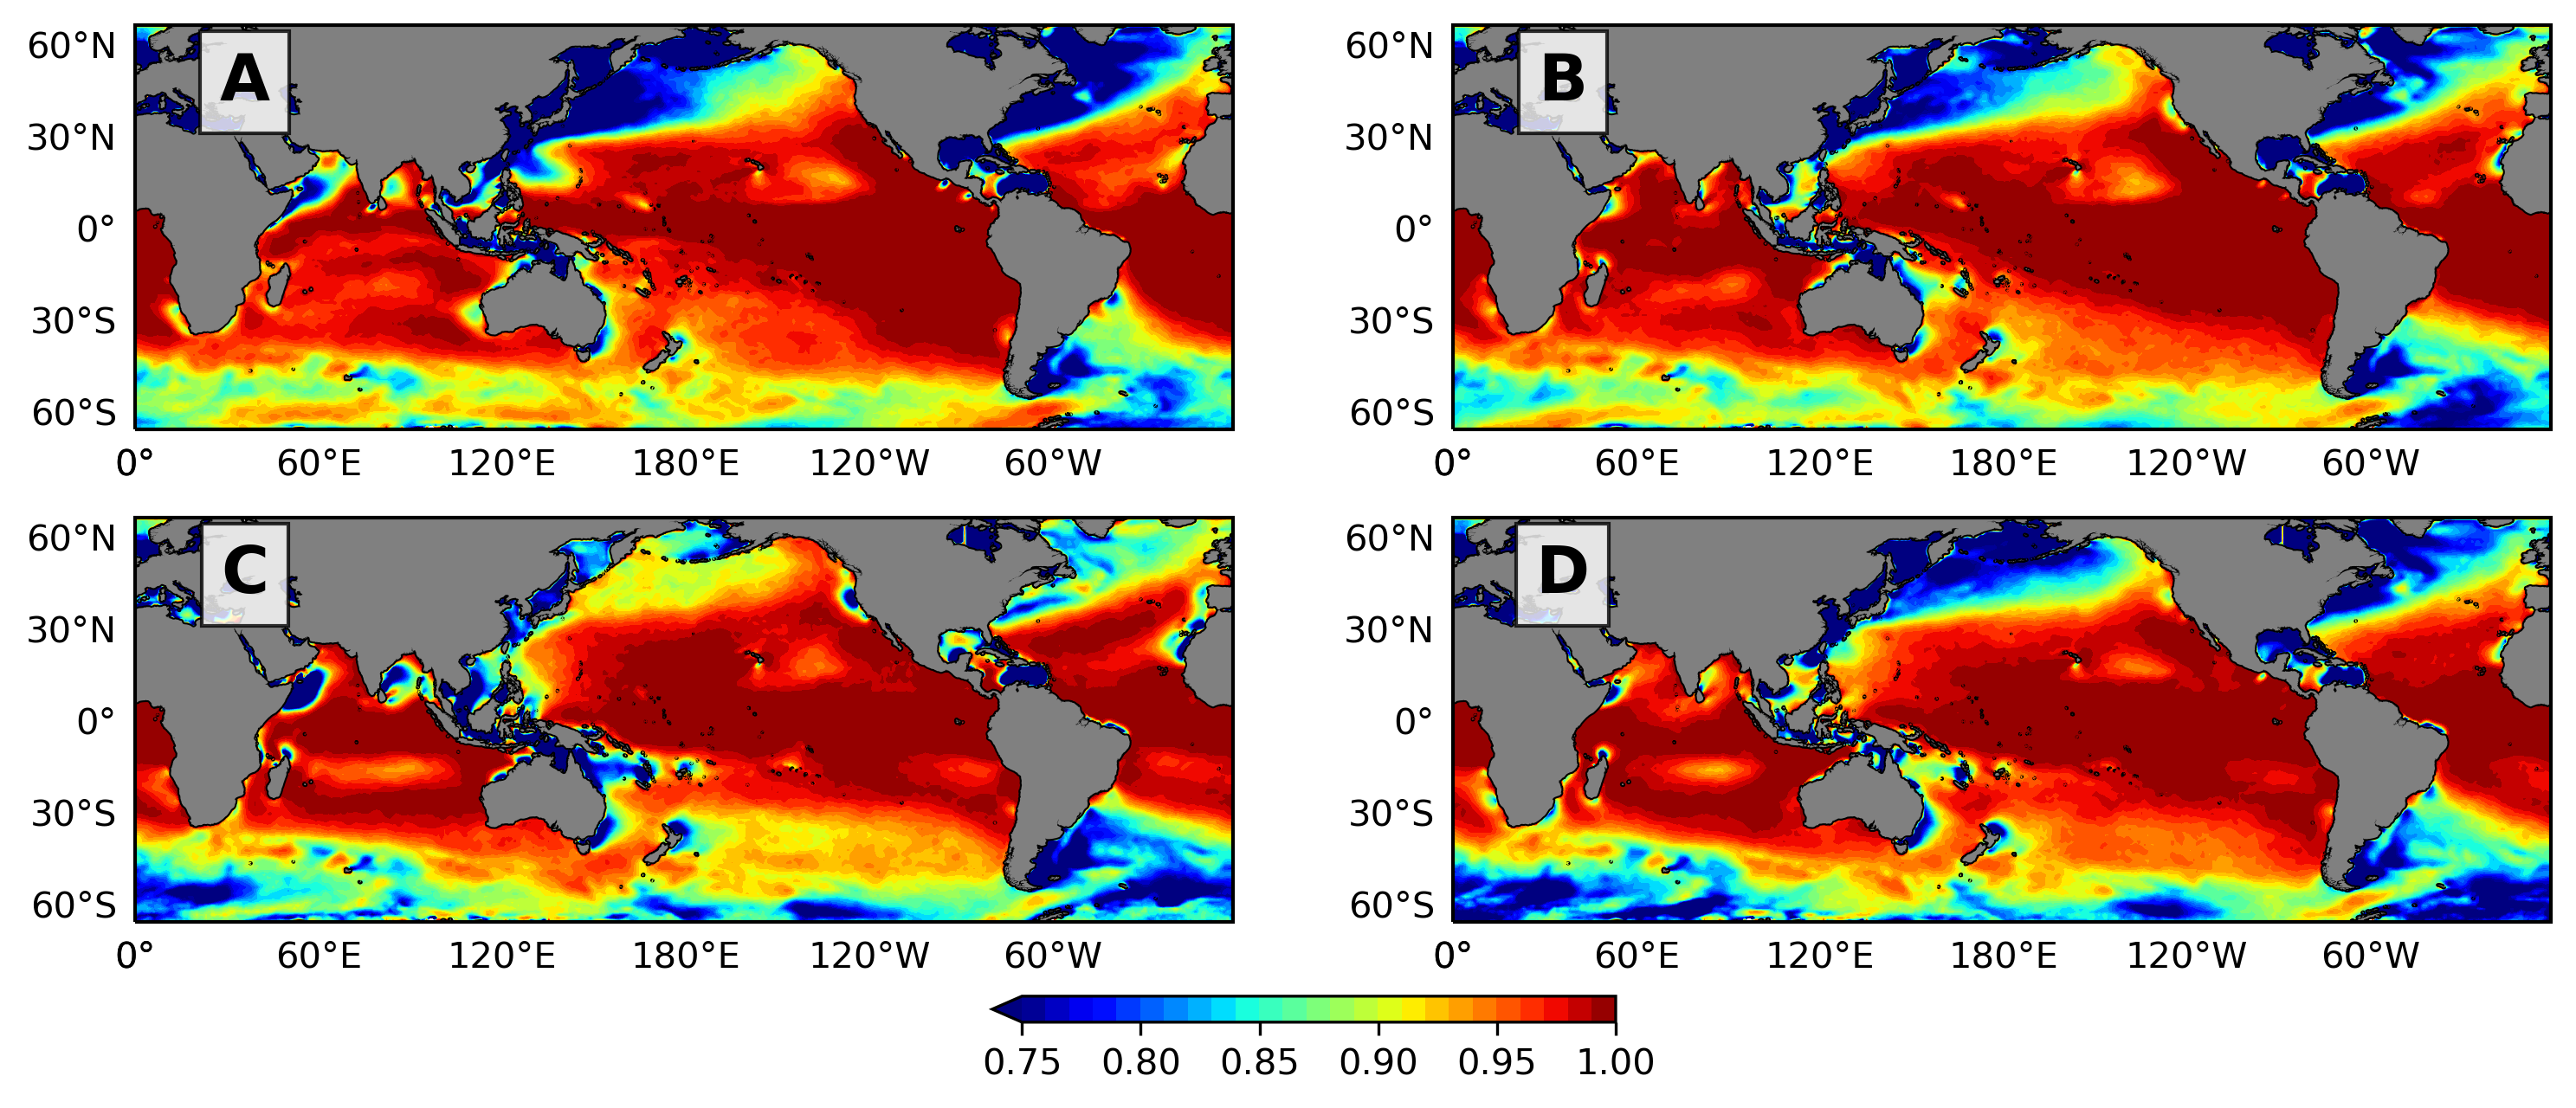
\includegraphics[width=1.0\textwidth]{figs/probability_of_swell/WW3_CFSR_prob_swell_seasons_2x2.png}
\caption{Seasonal progression of probability of swell using wave age criterion and WW3 peak frequency and WSP from January 1st, 1993 to December 31st, 2015 where (A) DJF, (B) MAM, (C) JJA, and (D) SON}.
\label{prob_swell_ww3}
\end{figure}

\section{Conclusion}

This study has analyzed the seasonal cycles of SWH and wind speed by least-squares fitting annual and semi-annual cycles to satellite observations.  In most of the ocean SWH is higher in winter, indicating a response to high-latitude winter storms that generate equatorward-propagating swell.  Exceptions occur in a few eastern boundary current regions, where strong local winds in spring or summer generate wind waves that are out of phase with the winter storms.  Using regional climatology analysis in 4$^{\circ}$ by 4$^{\circ}$ boxes, we find that in EBRs, the annual cycle of SWH can deviate from a sinusoidal annual cycle with winter maximum, instead indicating direct response to local WSP.  In EBRs the fraction of wave variability attributed to local wind events varies depending on local conditions. The waves within each EBR have low probability of swell during the spring and summer months of each hemisphere respectively. This implies that there is an increase in the number locally forced wind waves, supporting the hypothesis that the deviation from the SWH annual cycle results from wave that are locally forced by a local wind events.

Further research would include using spectral data from WW3 CFSR in order to separate wind-sea and swell characteristics in EBRs via spectral partitioning to further validate the claim that the deviation in the SWH seasonal cycle occurs from local wind events. In addition, local wind events should be further investigated to evaluate whether local winds result from the same atmospheric coastal topographic processes as in California. 

By improving our understanding of the SWH climate globally with respect to the effects of local wind events, wave models can more accurately model and anticipate increases in SWH. This would lead to an overall greater insight to ocean and atmospheric interactions including heat, momentum, and gas fluxes. 

%Other ideas for conclusion: 
% 1) Coastal infrastructure 
% 2) Application to wave current interaction 


%% ------------------------------------------------------------------------ %%

%%

%  Numbered lines in equations:
%  To add line numbers to lines in equations,
%  \begin{linenomath*}
%  \begin{equation}
%  \end{equation}
%  \end{linenomath*}



%% Enter Figures and Tables near as possible to where they are first mentioned:
%
% DO NOT USE \psfrag or \subfigure commands.
%
% Figure captions go below the figure.
% Table titles go above tables;  other caption information
%  should be placed in last line of the table, using
% \multicolumn2l{$^a$ This is a table note.}
%
%----------------
% EXAMPLE FIGURE
%
% \begin{figure}[h]
% \centering
% when using pdflatex, use pdf file:
% \includegraphics[width=20pc]{figsamp.pdf}
%
% when using dvips, use .eps file:
% \includegraphics[width=20pc]{figsamp.eps}
%
% \caption{Short caption}
% \label{figone}
%  \end{figure}
%
% ---------------
% EXAMPLE TABLE
%
% \begin{table}
% \caption{Time of the Transition Between Phase 1 and Phase 2$^{a}$}
% \centering
% \begin{tabular}{l c}
% \hline
%  Run  & Time (min)  \\
% \hline
%   $l1$  & 260   \\
%   $l2$  & 300   \\
%   $l3$  & 340   \\
%   $h1$  & 270   \\
%   $h2$  & 250   \\
%   $h3$  & 380   \\
%   $r1$  & 370   \\
%   $r2$  & 390   \\
% \hline
% \multicolumn{2}{l}{$^{a}$Footnote text here.}
% \end{tabular}
% \end{table}

%% SIDEWAYS FIGURE and TABLE
% AGU prefers the use of {sidewaystable} over {landscapetable} as it causes fewer problems.
%
% \begin{sidewaysfigure}
% \includegraphics[width=20pc]{figsamp}
% \caption{caption here}
% \label{newfig}
% \end{sidewaysfigure}
%
%  \begin{sidewaystable}
%  \caption{Caption here}
% \label{tab:signif_gap_clos}
%  \begin{tabular}{ccc}
% one&two&three\\
% four&five&six
%  \end{tabular}
%  \end{sidewaystable}

%% If using numbered lines, please surround equations with \begin{linenomath*}...\end{linenomath*}
%\begin{linenomath*}
%\begin{equation}
%y|{f} \sim g(m, \sigma),
%\end{equation}
%\end{linenomath*}

%%% End of body of article

%%%%%%%%%%%%%%%%%%%%%%%%%%%%%%%%
%% Optional Appendix goes here
%
% The \appendix command resets counters and redefines section heads
%
% After typing \appendix
%
%\section{Here Is Appendix Title}
% will show
% A: Here Is Appendix Title
%
%\appendix
%\section{Here is a sample appendix}

%%%%%%%%%%%%%%%%%%%%%%%%%%%%%%%%%%%%%%%%%%%%%%%%%%%%%%%%%%%%%%%%
%
% Optional Glossary, Notation or Acronym section goes here:
%
%%%%%%%%%%%%%%
% Glossary is only allowed in Reviews of Geophysics
%  \begin{glossary}
%  \term{Term}
%   Term Definition here
%  \term{Term}
%   Term Definition here
%  \term{Term}
%   Term Definition here
%  \end{glossary}

%
%%%%%%%%%%%%%%
% Acronyms
%   \begin{acronyms}
%   \acro{Acronym}
%   Definition here
%   \acro{EMOS}
%   Ensemble model output statistics
%   \acro{ECMWF}
%   Centre for Medium-Range Weather Forecasts
%   \end{acronyms}

%
%%%%%%%%%%%%%%
% Notation
%   \begin{notation}
%   \notation{$a+b$} Notation Definition here
%   \notation{$e=mc^2$}
%   Equation in German-born physicist Albert Einstein's theory of special
%  relativity that showed that the increased relativistic mass ($m$) of a
%  body comes from the energy of motion of the body—that is, its kinetic
%  energy ($E$)—divided by the speed of light squared ($c^2$).
%   \end{notation}




%%%%%%%%%%%%%%%%%%%%%%%%%%%%%%%%%%%%%%%%%%%%%%%%%%%%%%%%%%%%%%%%
%
%  ACKNOWLEDGMENTS
%
% The acknowledgments must list:
%
% >>>>	A statement that indicates to the reader where the data
% 	supporting the conclusions can be obtained (for example, in the
% 	references, tables, supporting information, and other databases).
%
% 	All funding sources related to this work from all authors
%
% 	Any real or perceived financial conflicts of interests for any
%	author
%
% 	Other affiliations for any author that may be perceived as
% 	having a conflict of interest with respect to the results of this
% 	paper.
%
%
% It is also the appropriate place to thank colleagues and other contributors.
% AGU does not normally allow dedications.


\acknowledgments
 Thank you to all institutions that provided data for my research project which include IFREMER, NASA Jet Propulsion Laboratory, and Remote Satellite Sensing. Thank you as well for the Hiestand Scholars program for funding my research over the summer of 2019.
 
 \noindent Thank you as well to my mentors Professor Sarah Gille and Bia Villas B\^oas for all the guidance and encouragement they has given me throughout this project. 

%% ------------------------------------------------------------------------ %%
%% References and Citations

%%%%%%%%%%%%%%%%%%%%%%%%%%%%%%%%%%%%%%%%%%%%%%%
% BibTeX is preferred:
%
%\section*{References}
%\noindent \bibentry{villas2017characterization}\\\\
%\bibentry{chen2002global}
\bibliography{agusample}

%
% no need to specify bibliographystyle
%%%%%%%%%%%%%%%%%%%%%%%%%%%%%%%%%%%%%%%%%%%%%%%



% Please use ONLY \citet and \citep for reference citations.
% DO NOT use other cite commands (e.g., \cite, \citeyear, \nocite, \citealp, etc.).
%% Example \citet and \citep:
%  ...as shown by \citet{Boug10}, \citet{Buiz07}, \citet{Fra10},
%  \citet{Ghel00}, and \citet{Leit74}.

%  ...as shown by \citep{Boug10}, \citep{Buiz07}, \citep{Fra10},
%  \citep{Ghel00, Leit74}.

%  ...has been shown \citep [e.g.,][]{Boug10,Buiz07,Fra10}.


\end{document}



More Information and Advice:

%% ------------------------------------------------------------------------ %%
%
%  SECTION HEADS
%
%% ------------------------------------------------------------------------ %%

% Capitalize the first letter of each word (except for
% prepositions, conjunctions, and articles that are
% three or fewer letters).

% AGU follows standard outline style; therefore, there cannot be a section 1 without
% a section 2, or a section 2.3.1 without a section 2.3.2.
% Please make sure your section numbers are balanced.
% ---------------
% Level 1 head
%
% Use the \section{} command to identify level 1 heads;
% type the appropriate head wording between the curly
% brackets, as shown below.
%
%An example:
%\section{Level 1 Head: Introduction}
%
% ---------------
% Level 2 head
%
% Use the \subsection{} command to identify level 2 heads.
%An example:
%\subsection{Level 2 Head}
%
% ---------------
% Level 3 head
%
% Use the \subsubsection{} command to identify level 3 heads
%An example:
%\subsubsection{Level 3 Head}
%
%---------------
% Level 4 head
%
% Use the \subsubsubsection{} command to identify level 3 heads
% An example:
%\subsubsubsection{Level 4 Head} An example.
%
%% ------------------------------------------------------------------------ %%
%
%  IN-TEXT LISTS
%
%% ------------------------------------------------------------------------ %%
%
% Do not use bulleted lists; enumerated lists are okay.
% \begin{enumerate}
% \item
% \item
% \item
% \end{enumerate}
%
%% ------------------------------------------------------------------------ %%
%
%  EQUATIONS
%
%% ------------------------------------------------------------------------ %%

% Single-line equations are centered.
% Equation arrays will appear left-aligned.

Math coded inside display math mode \[ ...\]
 will not be numbered, e.g.,:
 \[ x^2=y^2 + z^2\]

 Math coded inside \begin{equation} and \end{equation} will
 be automatically numbered, e.g.,:
 \begin{equation}
 x^2=y^2 + z^2
 \end{equation}


% To create multiline equations, use the
% \begin{eqnarray} and \end{eqnarray} environment
% as demonstrated below.
\begin{eqnarray}
  x_{1} & = & (x - x_{0}) \cos \Theta \nonumber \\
        && + (y - y_{0}) \sin \Theta  \nonumber \\
  y_{1} & = & -(x - x_{0}) \sin \Theta \nonumber \\
        && + (y - y_{0}) \cos \Theta.
\end{eqnarray}

%If you don't want an equation number, use the star form:
%\begin{eqnarray*}...\end{eqnarray*}

% Break each line at a sign of operation
% (+, -, etc.) if possible, with the sign of operation
% on the new line.

% Indent second and subsequent lines to align with
% the first character following the equal sign on the
% first line.

% Use an \hspace{} command to insert horizontal space
% into your equation if necessary. Place an appropriate
% unit of measure between the curly braces, e.g.
% \hspace{1in}; you may have to experiment to achieve
% the correct amount of space.


%% ------------------------------------------------------------------------ %%
%
%  EQUATION NUMBERING: COUNTER
%
%% ------------------------------------------------------------------------ %%

% You may change equation numbering by resetting
% the equation counter or by explicitly numbering
% an equation.

% To explicitly number an equation, type \eqnum{}
% (with the desired number between the brackets)
% after the \begin{equation} or \begin{eqnarray}
% command.  The \eqnum{} command will affect only
% the equation it appears with; LaTeX will number
% any equations appearing later in the manuscript
% according to the equation counter.
%

% If you have a multiline equation that needs only
% one equation number, use a \nonumber command in
% front of the double backslashes (\\) as shown in
% the multiline equation above.

% If you are using line numbers, remember to surround
% equations with \begin{linenomath*}...\end{linenomath*}

%  To add line numbers to lines in equations:
%  \begin{linenomath*}
%  \begin{equation}
%  \end{equation}
%  \end{linenomath*}
